\documentclass{article}
\usepackage[backend=bibtex]{biblatex}
\usepackage[utf8]{inputenc}
\usepackage[german]{babel}
\usepackage{caption}
\usepackage[skip=0.5ex]{subcaption}
\usepackage[left=3cm,right=3cm,top=2cm,bottom=2cm]{geometry}

\usepackage{color}
\usepackage{xcolor}
\usepackage{listings}
\definecolor{commentgreen}{rgb}{0.15,0.42,0.2}
\definecolor{codegray}{rgb}{0.5,0.5,0.5}
\definecolor{stringred}{rgb}{0.6,0.12,0.12}
\definecolor{functionblue}{rgb}{0,0,1}
\definecolor{backcolor}{rgb}{0.95,0.95,0.92}
\definecolor{linkcolor}{rgb}{0, 0.05, 0.3}


\usepackage{hyperref}
\hypersetup{
    colorlinks=true,
    linkcolor=linkcolor,
    filecolor=magenta,      
    urlcolor=cyan,
    pdftitle={GDV Summary},
    pdfpagemode=FullScreen,
    }
\usepackage{parskip} % do not indent first lines
\usepackage{bookmark}
\usepackage{booktabs}
\usepackage{textcomp}
\usepackage{array}
\usepackage{graphicx}
\usepackage{amsmath}
\usepackage{wrapfig} % wrap text around images/figures

\lstset{language=C++,
  commentstyle=\color{commentgreen},
  keywordstyle=\color{functionblue},
  numberstyle=\tiny\color{codegray},
  stringstyle=\color{stringred},
  basicstyle=\ttfamily\footnotesize,
  breakatwhitespace=false,         
  breaklines=true,                 
  captionpos=b,                    
  keepspaces=true,                 
  numbers=left,                    
  numbersep=5pt,                  
  showspaces=false,                
  showstringspaces=false,
  showtabs=false,                  
  tabsize=2
}



\newcommand{\quotes}[1]{''#1''}

\graphicspath{ {./images/} }

\begin{document}
\title{Summary\\Grundlagen Der Grafischen Datenverarbeitung - Meyer}
\author{Jonas Weßner}
\maketitle
\tableofcontents
\newpage				% Neue Seite nach TOC

\section{Graphische Programmierung}

\subsection{Definition von Graphischen Objekten}
Graphische Objekte bestehen letztendlich aus Punkten, die mit Kanten zu Dreiecken verbunden sind.\\
Man könnte auch denken, wieso denn nicht 4- oder 5-Ecke?\\
Jedes n-Eck, wobei 3 $\leq$ n, kann durch hinzufügen zusätzlicher Kanten nur mit Dreiecken dargestellt werden. Dreiecke haben zusätzlich den Vorteil, dass die eine Ebene im 3-dimensionalen kartesischen Koordinatensystem definieren. Dadurch kann das Dreieck als klarer Ebenenteil gezeichnet werden, wohingegen z.B. Vierecke nicht unbedingt in einer Ebene liegen und dadurch beim Zeichnen eventuell ohnehin als 2 getrennte Dreiecke gezeichnet werden müssten.\\

\subsection{Koordinatensysteme}
Wir betrachten das 3 dimensionale kartesische Koordinatensystem, welches als 3-dimensionales Orthogonalsystem definiert ist. Das bedeutet, dass es 3 Achsen gibt, die aus Vektoren bestehen, die paarweise Orthogonal zu sich stehen.\\
Wir unterscheiden weiter zwischen einem rechthändigen und linkshändigen Koordinatensystem, welche sich durch die Richtung der positiven z-Achse unterscheiden. Beim Rechtshändigen Koordinatensystem läuft die positive z-Achse zum betrachter hin, beim linkshändigen Koordinatensystem dementsprechend vom betrachter weg.
\\\\

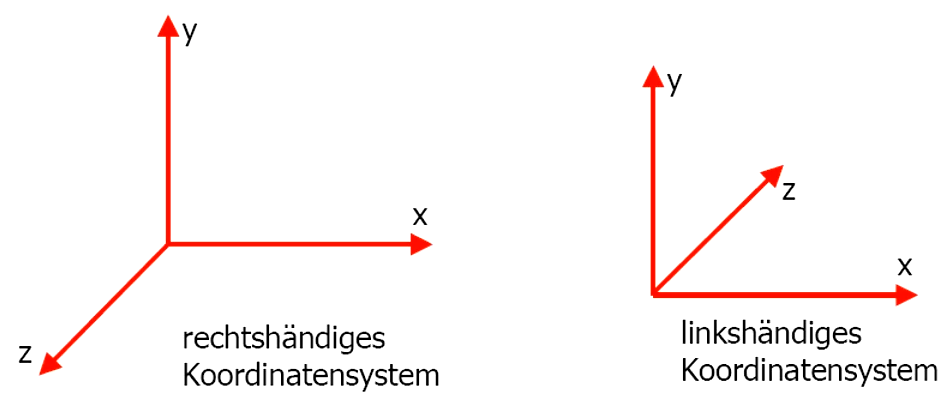
\includegraphics[width=400px]{images/Koordinatensysteme.png}

\subsection{Graphische Primitive in OpenGL}
In OpenGL können verschiedene \textit{Primitive} erzeugt werden. Das sind einfache Objekte, die von OpenGL auf Basis einzelner Punkte erzeugt werden. Diese kann man dann zusammenschließen, um komplexere Objekte zu erzeugen. Beispiele für Primitive sind hier gezeigt:

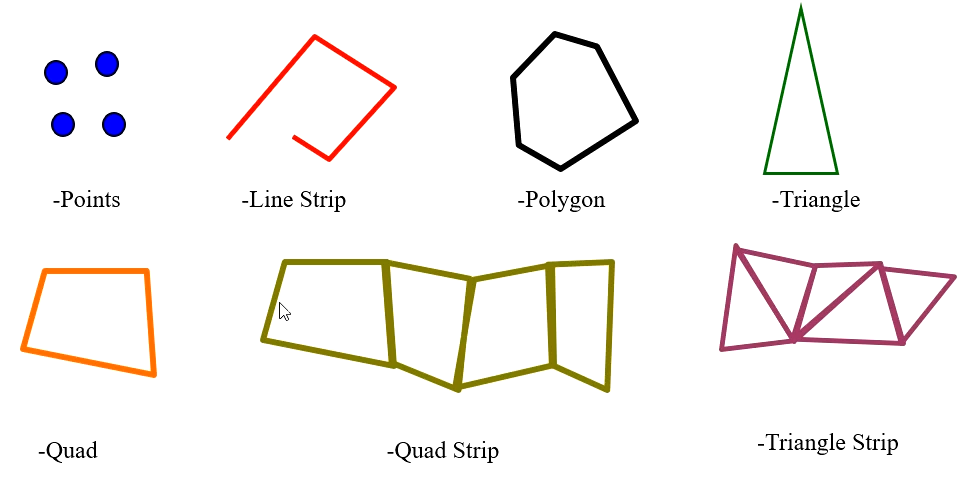
\includegraphics[width=400px]{images/openGlPrimitives.png}

\subsection{Transformationen Graphischer Objekte}
Jedes Objekt kann zunächst irgendwo in seinem Koordinatensystem definiert werden. Diese Platzierung nennt man nun die Platzierung in seinem \textit{lokalen Koordinatensystem}.\\
Durch verschiedene Transformationen kann das Objekt verändert werden, um seine Position, Ausrichtung und Größe zu verändern und schließlich im \textit{Weltkoordinatensystem} platziert werden.\\
Somit können Objekte einmalig durch geeignete Funktionen definiert werden und dann durch Transformationen für ihre aktuelle Verwendung angepasst werden. Die Transformationen sind konkret:
\begin{itemize}
    \item \textbf{Translation:} Verschiebung der Koordinaten eines Punktes. Dies entspricht der Addition eines Verschiebungsvektors auf den Ortsvektor des Punktes.
    \item \textbf{Rotation:} Drehen des Punktes um eine Koordinatenachse. Hierbei ist der Winkel entgegen des Uhrzeigersinns zu lesen.
    \item \textbf{Skalierung:} Multiplikation des Ortsvektors eines Punktes mit einem Skalar. Wird diese Operation für alle Punkte eines Objektes vorgenommen entsteht eine Stauchung oder Streckung entlang der Koordinatenachsen.
\end{itemize}

\subsection{Szenegraph}
Ein Szenegraph ist eine Datenstruktur, die eingesetzt werden kann, um mehrereg graphische Objekte zu einer Szene zusammenzuschließen.\\
Der Szenegraph ist ein gerichteter Zyklenfreier Graph. Das bedeutet, dass im Gegensatz zu einem Baum, ein Kindknoten auch mehrere Elternknoten haben kann, jedoch die Richtung der Abhängigkeiten einheitlich von Wurzel zu Blättern verläuft:
\\\\

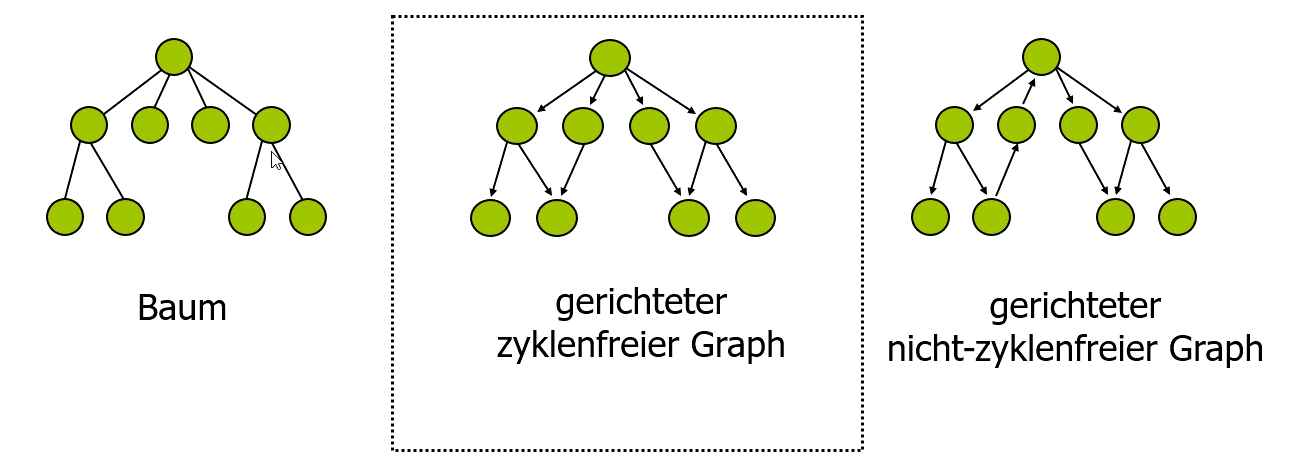
\includegraphics[width=400px]{images/gerichteterZyklenfreierGraph.png}

Die Knoten des Szenegraphen können Entweder Gruppen, Geometrien oder Transformationen sein:
\\


\includegraphics[height=50px]{images/Szenegraph_Knotentypen.png}
\\\\\\
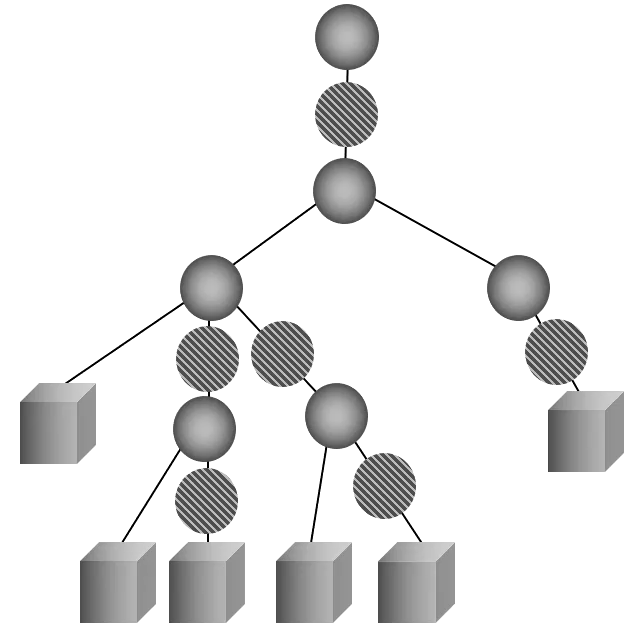
\includegraphics[width=200px]{images/Szenegraph_Beispiel.png}
\\\\

\textbf{Gruppen} bezeichnen hierbei zusammenfassungen von Punkten, die Graphische Objekte bilden. Transformationen beziehen sich dann auf alle Objekte, die im Szenegraphen unter ihnen liegen.\\
Dadurch kann man die Zusammenhänge komplexerer Objekte geeignet darstellen. Zum Beispiel soll eine Komplexe Figur, z.B. ein Mensch, sich generell im Raum bewegen können (Translation). Diese Translation wirkt sich dann auf alle Gruppen, die den Mensch bilden aus (als z.B. seinen Kopf, Rumpf, Arme und Beine). Der Mensch kann aber auch den Arm heben. Diese Translation soll sich dann also nur auf den Arm der Figur auswirken. Läuft der Mensch aber und hebt dabei seine Hand, so muss auf dem Arm offensichtlich sowohl die Translation des Körpers als auch die des Arms angewendet werden. So sieht man, dass der Arm im Szenegraphen also eine Gruppe sein muss, deren Eltengraphen die gesamte Figur "Mensch" ist.

\subsection{Arbeiten mit OpenGL}
OpenGL ist im Grunde eine Art Zustandsautomat und sehr explizit. Zunächst sind keine Einstellungen vorgenommen. Wird durch einen Funktionsaufruf eine Einstellung (z.B. der Farbe) Vorgenommen, so wird sie so lange beibehalten, bis sie geändert wird.\\
Ein weiteres Beispiel ist, dass der Bildschirm jedes Frame explizit gecleared werden muss, falls das vorherige Bild verworfen werden soll. Denn das vorherige Bild würde bestehen bleiben und nur die Stellen an denen Objekte gerendert werden aktualisiert werden.\\

\subsubsection*{Wie berechnet OpenGL Transformationen?}
Transformationen von Vektoren können mathematisch generell durchgeführt werden, indem eine Transformationsmatrix definiert wird, die mit dem Vektor multipliziert wird und so einen neuen Vektor ergibt. Sollen mehrere Transformationen auf einen Punkt angewendet werden, so muss ein Vektor also nacheinander mit mehreren Matrizen multipliziert werden. Dabei ist zu beachten, dass die Multiplikation von Matrizen nicht kommutativ aber assoziativ ist.\\

\[
    \begin{pmatrix}
        a & b & c \\
        d & e & f \\
        g & h & i
    \end{pmatrix}
    \cdot
    \left(
    \begin{pmatrix}
            a & b & c \\
            d & e & f \\
            g & h & i
        \end{pmatrix}
    \cdot
    \begin{pmatrix}
            a \\
            d \\
            g
        \end{pmatrix}
    \right)
    =
    \left(
    \begin{pmatrix}
            a & b & c \\
            d & e & f \\
            g & h & i
        \end{pmatrix}
    \cdot
    \begin{pmatrix}
            a & b & c \\
            d & e & f \\
            g & h & i
        \end{pmatrix}
    \right)
    \cdot
    \begin{pmatrix}
        a \\
        d \\
        g
    \end{pmatrix}
\]
\\

OpenGL geht so vor, dass es immer, wenn eine Transformation definiert wird, diese mit der aktuellen globalen Tranformationsmatrix multipliziert (Zu Beginn ist diese Matrix die Dreidimensionale Einheitmatrix). Immer wenn dann ein Objekt definiert wird, wird diese aktuelle Transformationsmatrix auf das Objekt angewendet.\\
Weil die Multiplikation assoziativ ist, entspricht das Ergebnis der Multiplikation in jedem Fall dem Ergebnis, das entsteht, wenn man den Vektor von rechts nach links mit den Matrizen multipliziert. Will man also eine bestimmte Transformation vor einer anderen durchführen, so muss sie weiter rechts stehen, um früher angewendet zu werden.
\subsubsection*{Matrizenstack}
Neben der aktuellen Transformationsmatrix, die sich immer auf die aktuell definierten Objekte bezieht, speichert OpenGL auch noch einen sogenannten Matrizenstack.\\
Ein Aufruf von \textit{glPushMatrix()} legt die aktuelle Transformationsmatrix auf dem Stack ab. Die Matrix wird aber auch als aktuelle Matrix weiter verwendet.\\
Ein Aufruf von \textit{glPopMatrix()} ersetzt die aktuelle Transformationsmatrix durch die zuletzt gepushte Matrix und entfernt sie vom Matrizenstack.\\
Somit kann also eine Matrix gesichert und später wiederverwendet werden, wie etwa bei Unterprogrammaufrufen in ASM, wenn man zunächst die aktuellen Register auf dem Stack rettet.\\
Zum Beispiel könnte man sich vorstellen, dass ein um 45 Grad gedrehter Würfel erzeugt werden soll, der außerdem um 2 Längen entlang der negativen y-Achse verschoben ist und ein Würfel im Ursprung des Koordinatensystem gezeichnet werden soll. Wenn man nicht den Matrizenstack nutzt würde das in etwa so aussehen:
\begin{itemize}
    \item glRotatef(45, 1.0, 0.0, 0.0);
    \item glTranslatef(0.0, -2.0, 0.0);
    \item Cube();
    \item glRotatef(-45, 1.0, 0.0, 0.0);
    \item glTranslatef(0.0, 2.0, 0.0);
    \item Cube();
\end{itemize}
Mit Benutzung des Matrizenstacks ist das Wiederherstellend er ursprünglichen Transformationsmatrix einfacher:
\begin{itemize}
    \item glPushMatrix();
    \item glRotatef(45, 1.0, 0.0, 0.0);
    \item glTranslatef(0.0, -2.0, 0.0);
    \item Cube();
    \item glPopMatrix();
    \item Cube();
\end{itemize}

\subsubsection*{Definition von Dreiecksstreifen}
Wenn komplexe Objekte aus Dreiecken gebildet werden sollen, dann sind viele Eckpunkte eines vorherigen Dreiecks wieder ein Eckpunkt eines folgenden Dreiecks und damit die definition und Speicherung dieses redundant. Somit kann durch das Benutzen von  \textit{GL\_TRIANGLE\_STRIP}s effizienter vorgegangen werden.\\

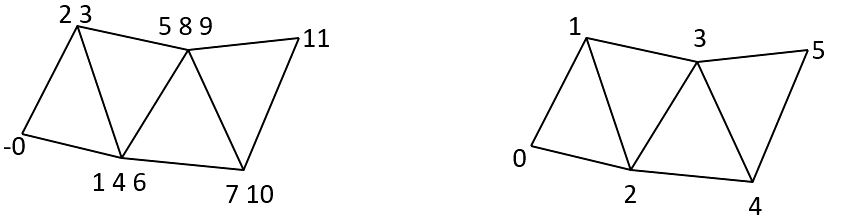
\includegraphics[width=350px]{images/glTriangleStrip.png}

\subsubsection*{Definition von Farben und Texturen}
Farben und Texturen werden jeweils global umgestellt und gelten dann für alle folgenden Punkte (siehe Zustandsautomat). Flächen oder Linien, die letztendlich durch die Verbindung von Punkten entstehen erhalten dann die lineare Interpolation der Farb und Texturwerte der zugehörigen Punkte:\\

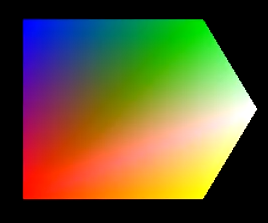
\includegraphics[height=80px]{images/openGlColors.png}

\subsubsection*{Rotation von Objekten um sich selbst}
Soll ein Objekt um seinen eigenen Mittelpunkt gedreht werden, so kann dieses Objekt zunächst in den Ursprung des Koordinatensystems bewegt werden, dann die Rotation durchgeführt werden und dann muss es wieder an seinen ursprünglichen Platz zurückbewegt werden.\\
Auf diese Weise kann der Standort des Objektes vor der Rotation erhalten bleiben.\\
Hierbei ist auch zu beachten, dass die Rücktranslation zuerst angegeben werden muss, dann die Rotation und dann die Translation, da wie gesagt die zuletzt angegebene Transformation zuerst angewendet wird.
\newpage
\section{Abbilden Graphischer Objekte}

\subsection{Kameramodell}

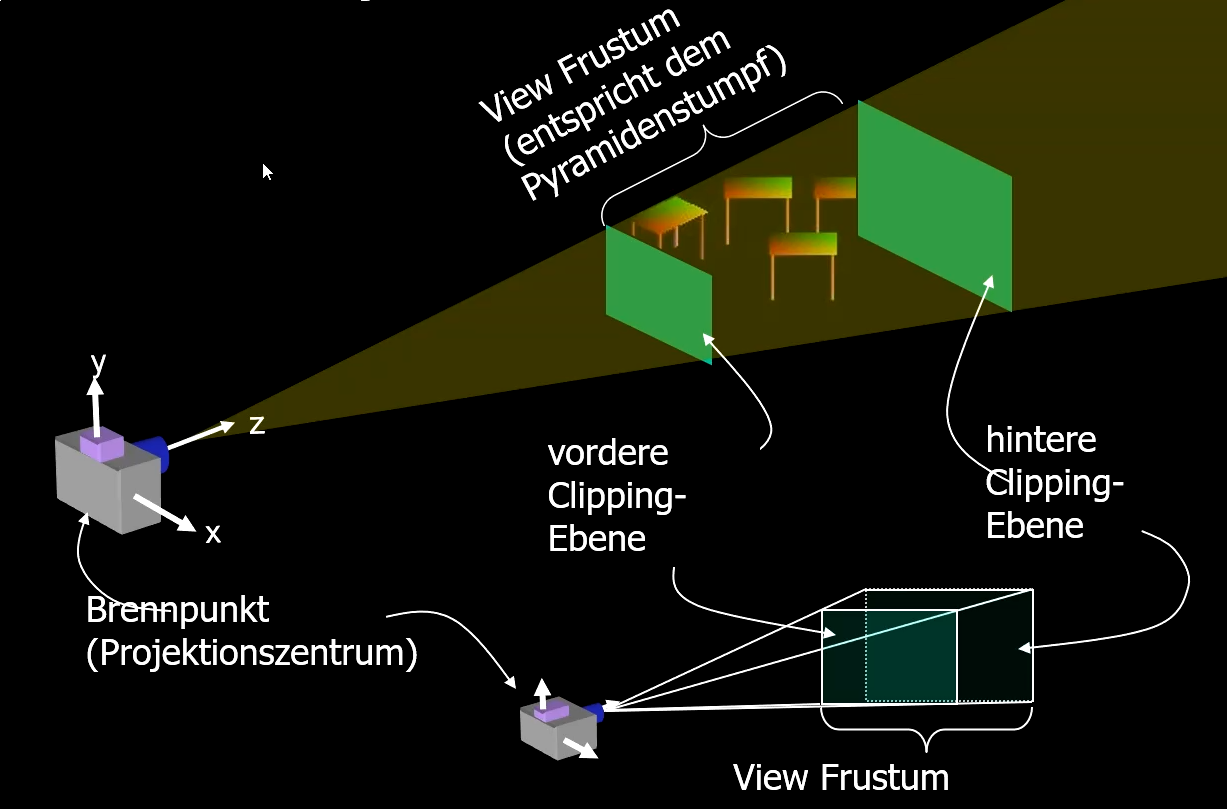
\includegraphics[width=400px]{images/kameramodell.png}

\vspace{10px}

Im vorherigen Kapitel haben wir gelernt, wie man graphische Objekte im ''Weltkoordinatensystem'' also im globalen Koordinatensystem erzeugen kann. Die Abbildung dieser 3-dimensionalen Welt auf dem 2-dimensionalen Bildschirm hängt jetzt von der Position des Betrachters, sowie einigen weiteren Parametern ab.\\
Dazu kann man sich zu visualisierung das folgende Kameramodell vorstellen:\\
Die Kamera steht an einer beliebigen Position im Weltkoordinatensystem, die durch einen Ortsvektor bestimmt wird. Sie ist in eine bestimmte Richtung gerichtet, die durch einen Punkt, auf den sie gerichtet ist, definiert ist. Dieser Punkt ist wiederum durch seinen eigenen Ortsvektor im Weltkoordinatensystem fest definiert. Wenn sich die Kamera bewegt, dann ändert sich ihre Blickrichtung so, dass sie weiterhin auf den Blickpunkt zeigt.\\
Die Kamera hat einen Öffnungswinkel, der den Winkel bezeichnet, den das gelbe Dreieck an der Ecke hat, die sich an der Kamera befindet. Wenn der Öffnungswinkel größer ist, ist also das Sichtfeld breiter.\\
Die vordere und hintere Clipping-Ebenen begrenzen das Feld, das gerendert wird nach vorne und hinten (von der Kamera aus gesehen). Die Clipping Ebenen sind relativ zur Kamera positioniert, bewegen sich also mit, wenn sich die Kamera bewegt.\\
Somit wird letztendlich der gelbe Pyramidenstumpf, den man auch View Frustum, zwischen den beiden grünen Ebenen gerendert. Nun bleibt noch die Frage, wie man es schaffen kann, dass die 3-dimensionale Welt auf einen 2-Dimensionalen Bildschirm abgebildet wird und dabei trotzdem realistisch aussieht. Das wollen wir als Nächstes betrachten.

\subsection{Perspektivische Projektion}

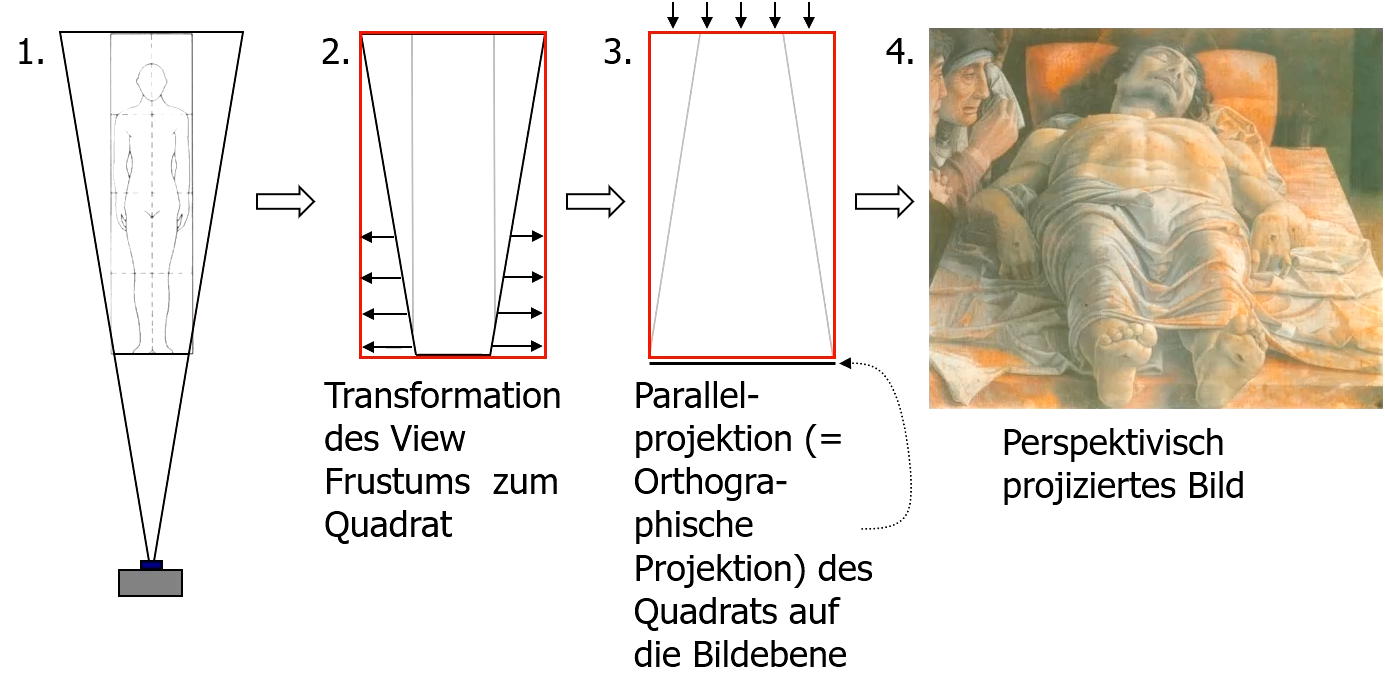
\includegraphics[width=400px]{images/perspektivischeProjektion.png}

\vspace{10px}

Betrachtet man Bilder von Kameras (oder das eigene Sichtbild, das auf die Netzhaut des Auges projiziert wird), so stellt man schnell fest, dass Dinge, die Nahe am Betrachter sind, größer sind, als Dinge, die weiter entfernt sind. Dieses Verhalten können wir auch bei der Projektion in der Computergraphik herstellen, um realistische Bilder zu erzeugen.\\
\begin{enumerate}
    \item Zunächst wird mithilfe des Kameramodells aus dem vorherigen Abschnitt der zu rendernde Bereich bestimmt. In der Realität wäre das der Bereich, dessen Lichtstrahlen durch ihre Position bedingt durch die Pupille auf die Netzhaut gelangen können (nur in der Realität ist der Bereich nicht nach vorne und hinten begrenzt). Das Bett, auf dem der Mensch auf dem Bild liegt bedeckt also den kompletten vorderen Rand des View Frustums und hinten ist neben dem Bett auch noch ein Stück der Umgebung im Bild.
    \item Nun wird der Pyramidenstumpf mittels einer Transformation so verzerrt, dass sich ein Quader (nicht Quadrat wie auf dem Bild steht!) bildet. Dadurch werden Objekte, die näher sind breiter. Auf diese Weise kann man sich auch leicht vorstellen, dass, wenn man den Öffnungswinkel der Kamera vergrößert, dieser Effekt stärker wird, d.h. weiter entfernte Objekte wirken dann noch kleiner und nähere noch größer. Auf unserem Bild wird das Bett an seiner vorderen Kante gestreckt, sodass seine eigentlich parallelen Seitenkanten auf dem Bild nach hinten spitz zusammenlaufen.
    \item Nun wird eine Parallelprojektion/orthographische Projektion durchgeführt, bei der der Quader auf ein Rechteck (das eigentliche Bild) abgebildet wird. Dabei ist es intuitiv notwendig, dass weiter vorne liegende Objekte weiter hinten liegende Objekte überlagern müssen.
\end{enumerate}

\subsubsection*{Projektionsmöglichkeiten}


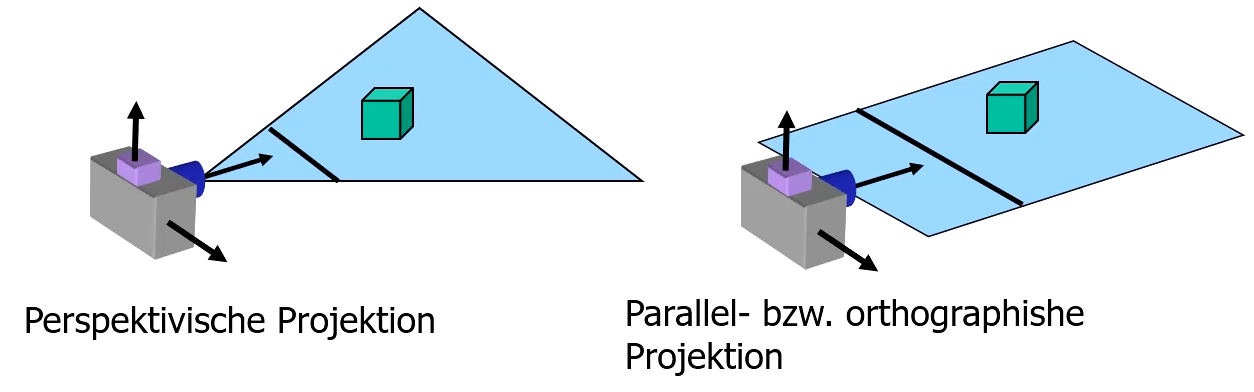
\includegraphics[width=300px]{images/projektionsmoeglichkeiten.png}


OpenGL biete neben der perspektivischen Projektion auch noch die Möglichkeit Parallelprojektion/orthographische Projektion zu benutzen. Diese Projektionsmethode haben wir bereits kennengelernt, als wir die perspektivische Projektion betrachtet haben, da sie immer notwendig ist, um den 3-dimensionalen Raum auf ein 2-dimensionales Bild zu projizieren. Benutzt man nur Parallelprojektion (d.h. nicht bloß im Rahmen der ''Toolchain''), dann ist eigentlich die Kamera, die auf dem Bild eingezeichnet ist, überflüssig. Alle Objekte werden dann direkt auf die schwarze Linie, die das Bild darstellen soll, abgebildet. In der Anwendung bedeutet das, dass die Perspektive alleine durch die Position und Größe der Clipping-Ebenen definiert ist und jedes Objekt unabhängig von seiner Position im Bild genau die größe hat, die es in der Realität hat (aber man kann das Bild danach natürlich noch skalieren). Das Größenverhältnis von Objekten bleibt auf dem Bild so, wie es in der Realität ist. Dieses Verhalten ist unnatürlich. Dabei entstehen Bilder, die ähnlich sind wie das folgende:

\vspace{10px}

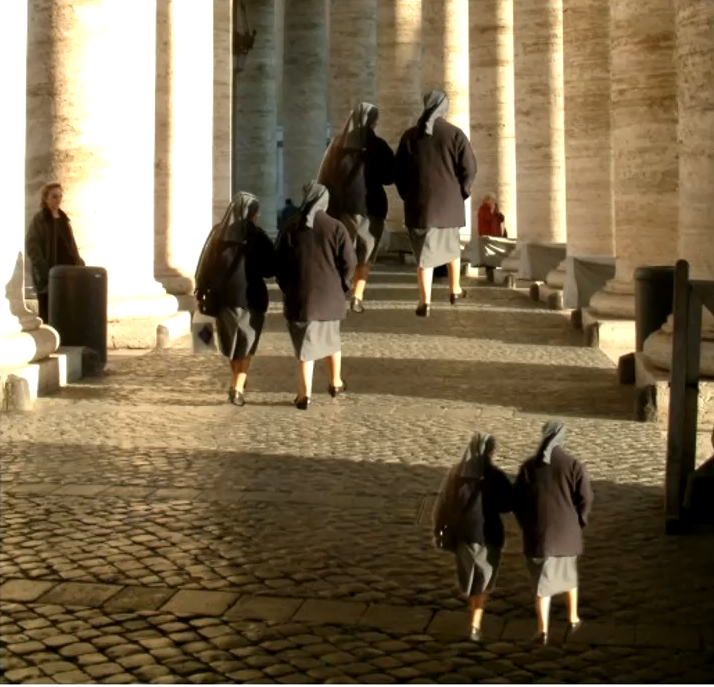
\includegraphics[width=300px]{images/perspektivischeWahrnehmung.png}

\subsection{Projektionsverfahren in OpenGL}
Die Projektionsmöglichkeiten werden in OpenGL auch über die Multiplikation der aktuellen Matrix mit Transformationsmatrizen geregelt. Dafür gibt es bestimmte Funktionen:

\subsubsection*{Orthographische Projektion}

\lstinputlisting[language=c++]{src/snippets/glOrtho.c++}

Der Funktionsaufruf erstellt eine Matrix für eine orthographische Projektion und multipliziert sie mit der aktuellen Matrix, indem er statt einem View Frustum einen View Quader definiert. Der ganze Inhalt des Quaders wird also auf die near Clipping Plane projiziert, welche dann auf das Ausgabefenster gemapt wird.

\begin{itemize}
    \item \textbf{left, bottom} geben den linken unteren Eckpunkt und \textbf{right, top} den rechten oberen Eckpunkt für die Clipping Planes an. Mittels der Information über die 2 Diagonalen Punkte und der Information, dass ein Rechteck entstehen soll, ist die größe des Rechtecks definiert
    \item \textbf{near} und \textbf{far} beschreiben die Entfernung zum Betrachter mit denen die zwei identisch großen Clipping Planes platziert werden sollen
    \item Die Clipping Planes werden so ausgerichtet, dass der Betrachter orthogonal auf sie schaut.
\end{itemize}

\subsubsection*{Perspektivische Projektion}

\lstinputlisting[]{src/snippets/gluPerspective.cpp}

Diese Funktion definiert ein View Frustum im Weltkoordinatensystem, generiert daraus eine Transformationsmatrix und multipliziert sie mit der aktuellen Matrix.

\begin{itemize}
    \item \textbf{fovy} gibt den Öffnungswinkel in y-Richtung an.
    \item \textbf{aspect} gibt das Seitenverhältnis $x \div y$ an.
    \item \textbf{zNear} bezeichnet die Distanz des Betrachters zur near-clipping-plane
    \item \textbf{zFar} bezeichnet die Distanz des Betrachters zur far-clipping-plane
\end{itemize}

Die konkreten Seitenlängen lassen sich für jeden Teil des Frustums also durch den Öffnungswinkel, die Entfernung, das Seitenverhältnis und den aktuellen Standpunkt des Beobachters (Standardmäßig im Ursprung, ansonsten mit \textit{gluLookAt} veränderbar) bestimmen. Somit ist das Frustum vollständig definiert.

\subsubsection*{Bewegung des Betrachters}

\lstinputlisting{src/snippets/gluLookAt.cpp}

Diese Funktion ermöglicht es den Betrachter zu verschieben und seine Ausrichtung zu verändern.\\
Wenn der Betrachter verschoben wird, \textbf{bewegen sich die Clipping-Planes mit ihm.}

\begin{itemize}
    \item \textbf{eyeX, eyeY, eyeZ} beschreiben den Ortsvektor der Linse des Betrachters
    \item \textbf{centerX, centerY, centerZ} beschreiben den Ortsvektor des Punktes auf die der Betrachter schaut
    \item \textbf{upX, upY, upZ} beschreibt den Ortsvektor des Punktes, der vom Betrachter aus als oben betrachtet wird
\end{itemize}


\newpage

\section{Mathematische Grundlagen}

Die Transformationen, die wir genauer betrachten wollen sind die Translation (Verschiebung), die Transformation (Größenänderung) und die Rotation (Drehung). Diese Transformationen nennt man auch affine Abbildungen. Das bedeutet, dass:
\begin{enumerate}
    \item Die Bildpunkte von Punkten, die auf einer Gerade liegen, liegen wieder auf einer Geraden.
    \item Die Bilder von parallelen Geraden sind wieder Parallel.
    \item Die Größenverhältnisse der Bildpunkte stimmen mit denen der ursprünglichen Punkte überein.
\end{enumerate}

Wir wollen uns nun ansehen, wie diese Transformationen mathematisch umgesetzt werden.

\subsection{Skalierung}
Die Skalierung eines Vektors $\vec{x}$ wird beschrieben durch die Multiplikation mit einem Skalar y:

\[
    \begin{pmatrix}
        x_{1} \\
        x_{2} \\
        x_{3}
    \end{pmatrix}
    \cdot
    y
\]


Auf diese Weise wird jede Komponente von $\vec{x}$ mit dem gleichen Wert y multipliziert. Um mehr Flexibilität zu erlangen und Objekte auch in verschiedene Achsenrichtungen unterschiedlich skalieren zu können, können wir die Skalierung auch als Matrix $Y$ definieren. Diese Methode wird auch von OpenGL verwendet. Wenn wir eine Transformation definieren wird die aktuelle Matrix $A$ mit einer Transformationsmatrix $X$ multipliziert. Diese werden dann mit den Ortsvektoren $\vec{x_{i}}$ aller Punkte der Objekte multipliziert.

\[
    A
    \cdot
    \begin{pmatrix}
        y_{1} & 0     & 0     \\
        0     & y_{2} & 0     \\
        0     & 0     & 0_{3} \\
    \end{pmatrix}
    \cdot
    \begin{pmatrix}
        x_{1} \\
        x_{2} \\
        x_{3}
    \end{pmatrix}
\]


\subsection{Rotation}

Die Rotation/Drehung wird ebenfalls durch die Multiplikation mit einer Matrix beschrieben. Die Komponente der Vektoren, mit denen die Matrix multipliziert wird, um die sich gedreht wird, darf nicht verändert werden. muss der Zeilenvektor, an dieser Stelle die Komponenten haben, die die Einheitsmatrix an dieser Stelle hätte.

Rotation um $\alpha$ gegen den Uhrzeigersinn um die x Achse:

\[
    A(\alpha)
    \cdot
    \begin{pmatrix}
        1 & 0          & 0           \\
        0 & \cos\alpha & -\sin\alpha \\
        0 & \sin\alpha & \cos\alpha  \\
    \end{pmatrix}
\]

Rotation um $\alpha$ gegen den Uhrzeigersinn um  die y-Achse:

\[
    A(\alpha)
    \cdot
    \begin{pmatrix}
        \cos\alpha & 0 & -\sin\alpha \\
        0          & 1 & 0           \\
        \sin\alpha & 0 & \cos\alpha  \\
    \end{pmatrix}
\]

Rotation um $\alpha$ gegen den Uhrzeigersinn um  die z-Achse:

\[
    A(\alpha)
    \cdot
    \begin{pmatrix}
        \cos\alpha & -\sin\alpha & 0 \\
        \sin\alpha & \cos\alpha  & 0 \\
        0          & 0           & 1 \\
    \end{pmatrix}
\]

\subsection{Translation}

Die Translation ist auf den ersten Blick eine Vektoraddition eines Ortsvektors $\vec{v}$ mit einem Translationsvektors $\vec{t}$:

\begin{equation}
    \vec{x}
    +
    \vec{t}
    =
    \begin{pmatrix}
        v_{1} \\
        v_{2} \\
        v_{3}
    \end{pmatrix}
    +
    \begin{pmatrix}
        t_{1} \\
        t_{2} \\
        t_{3}
    \end{pmatrix}
    =
    \begin{pmatrix}
        v_{1} + t_{1} \\
        v_{2} + t_{2} \\
        v_{3} + t_{3}
    \end{pmatrix}
\end{equation}

Während diese Herangehensweise für das Rechnen mit der Hand gut funktioniert, haben wir bei der maschinellen Berechnung ein Design-Problem. Denn die anderen beiden Transformationen, Skalierung und Rotation, können wir als Multiplikationen mit einer Matrix darstellen. OpenGL kann also alle Transformationsmatrizen multiplizieren und somit eine akkumulierte Matrix berechnen, die dann auf alle Punkte der Objekte angewandt wird. Wenn wir die Translation als addition mit einem Translationsvektor $\vec{y}$ beschreiben, müsste OpenGL zusätzlich zur akkumulierten Matrix auch noch einen akkumulierten Translationsvektor speichern, auf den alle Transformationen aufaddiert werden. Damit OpenGL trotzdem bloß mit Matrixmultiplikation rechnen kann, werden Homogene Koordinaten verwendet.\\
Homogene Koordinaten beschreiben das Erweitern der Vektoren und Matrizen eines bestimmten Vektorraums (hier der 3-dimensionale Vektorraum), um die Koordinaten einer weiteren Dimension. Dabei erweitern vir alle Vektoren $\vec{v}$ um eine Koordinate $v_{4}=1$. Alle Matrizen $M$ werden mit den Koordinaten der 4-dimensionalen Einheitsmatrix erweitert. Dabei können aber Koordinaten $M_{14}, M_{24}, M_{34}$ durch die Komponenten des Translationsvektors $\vec{t}$ aus (1) ersetzt werden.

\begin{equation}
    \vec{v}
    =
    \begin{pmatrix}
        v_{1} \\
        v_{2} \\
        v_{3}
    \end{pmatrix}
    \rightarrow
    \vec{v'}
    =
    \begin{pmatrix}
        v_{1} \\
        v_{2} \\
        v_{3} \\
        1
    \end{pmatrix}
\end{equation}

\[
    M
    =
    \begin{pmatrix}
        M_{11} & M_{12} & M_{13} \\
        M_{21} & M_{22} & M_{23} \\
        M_{31} & M_{32} & M_{33} \\
    \end{pmatrix}
    \rightarrow
    M'
    =
    \begin{pmatrix}
        M_{11} & M_{12} & M_{13} & t_{1} \\
        M_{21} & M_{22} & M_{23} & t_{3} \\
        M_{31} & M_{32} & M_{33} & t_{3} \\
        0      & 0      & 0      & 1
    \end{pmatrix}
\]

Mithilfe dieser Erweiterung können wir nun auch die Translation als Matrixmultiplikation darstellen. Denn bei der Multiplikation der Matrix $M'$ mit dem Vektor $\vec{v'}$ entsteht ein Vektor $\vec{v'_{M'}}$, der identisch zu dem Vektor $\vec{v_{Mt}}$ ist, der entsteht, wenn man zunächst die Multiplikation mit $M$ und dann die Addition mit $\vec{t}$ durchgeführt hätte und ihn um eine homogene Koordinate erweitert.

\begin{equation}
    M
    \cdot
    \vec{v}
    +
    \vec{t}
    \rightarrow
    M'
    \cdot
    \vec{v'}
    =
    \begin{pmatrix}
        M_{11} & M_{12} & M_{13} & t_{1} \\
        M_{21} & M_{22} & M_{23} & t_{3} \\
        M_{31} & M_{32} & M_{33} & t_{3} \\
        0      & 0      & 0      & 1
    \end{pmatrix}
    \cdot
    \begin{pmatrix}
        v_{1} \\
        v_{2} \\
        v_{3} \\
        1
    \end{pmatrix}
    =
    \begin{pmatrix}
        v_{1} \cdot M_{11} + v_{2} \cdot M_{12} + v_{3} \cdot M_{13} + \boldsymbol{t_{1}} \\
        v_{1} \cdot M_{21} + v_{2} \cdot M_{22} + v_{3} \cdot M_{23} + \boldsymbol{t_{2}} \\
        v_{1} \cdot M_{31} + v_{2} \cdot M_{32} + v_{3} \cdot M_{33} + \boldsymbol{t_{3}} \\
        1
    \end{pmatrix}
\end{equation}
\section{Koordinatensysteme}

In diesem Kapitel werden wir sehen, wie wir in speziellen Koordinatensystemen bestimmte geometrische Objekte einfacher Darstellen können. Der Grund ist, das wir in der Computergrafik besser mit geraden Strecken rechnen können als mit kontinuierlichen Bögen. Die im Folgenden gezeigten Koordinatensysteme ermöglichen die Darstellung von rundungsintensiven Geometrien als Strecken oder n-Ecke. Dazu wird die Bedeutung der Achsen des kartesischen Koordinatensystems verändert.

\subsection{Polarkoordinatensystem}

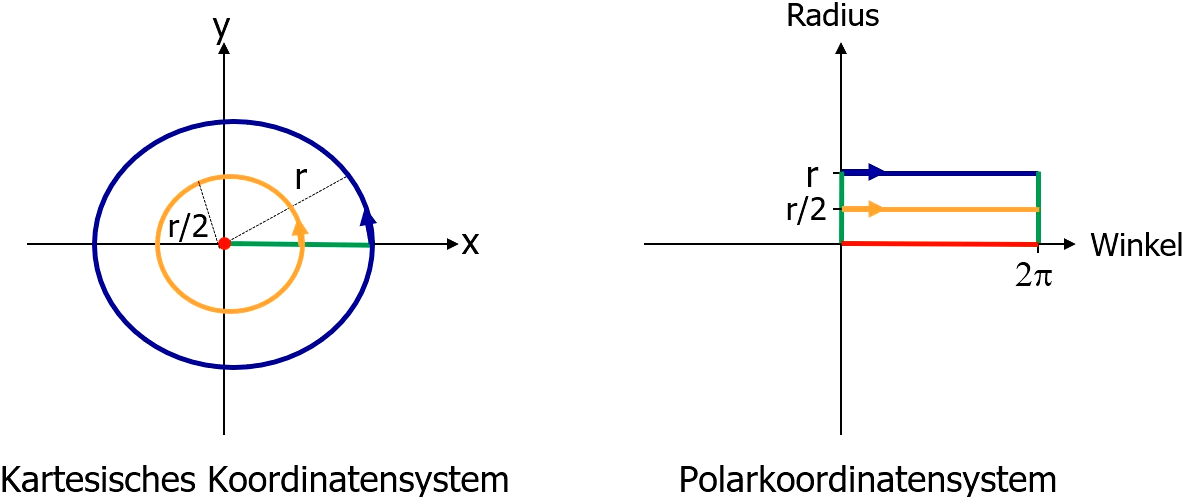
\includegraphics[width=400px]{Polarkoordinatensystem1.png}

Das Polarkoordinatensystem ist ein 2-dimensionales Koordinatensystem. Bei der Übertragung eines Punktes P aus dem kartesischen Koordinatensystems ins Polarkoordinatensystem wird die Entfernung des Punktes P zum Ursprung auf die eine Achse übertragen (Radius $r$). Auf die andere Achse wird der Winkel ($\alpha$) übertragen, den die positive x-Achse mit der Strecke zwischen dem Punkt P und dem Ursprung gegen den Uhrzeigersinn bildet. Dementsprechend sind die Umrechnungsregeln wie folgt definiert:\\

Von kartesischem Koordinatensystem zu Polarkoordinatensystem:\\
\begin{math}
    r = \sqrt{x^2 + y^2}\\
    \alpha = \arctan(y / x)
\end{math}

Von Polarkoordinatensystem zu kartesischem Koordinatensystem, mittels der Gesetzte für trigon. Funktionen entsprechend umgeformt, sodass die rechte Seite nur die Achsen des Polarkoordinatensystem enthält:\\
\begin{math}
    x = \cos{\alpha} \cdot r\\
    y = \sin(\alpha) \cdot r
\end{math}

Mittels dieser Definition können wir nun nun viele geometrische Formen, die normalerweise rundungen haben, als eckige Formen darstellen. Es folgt noch ein Beispiel.

\subsubsection{Kreisauschnitt im Polarkoordinatensystem}

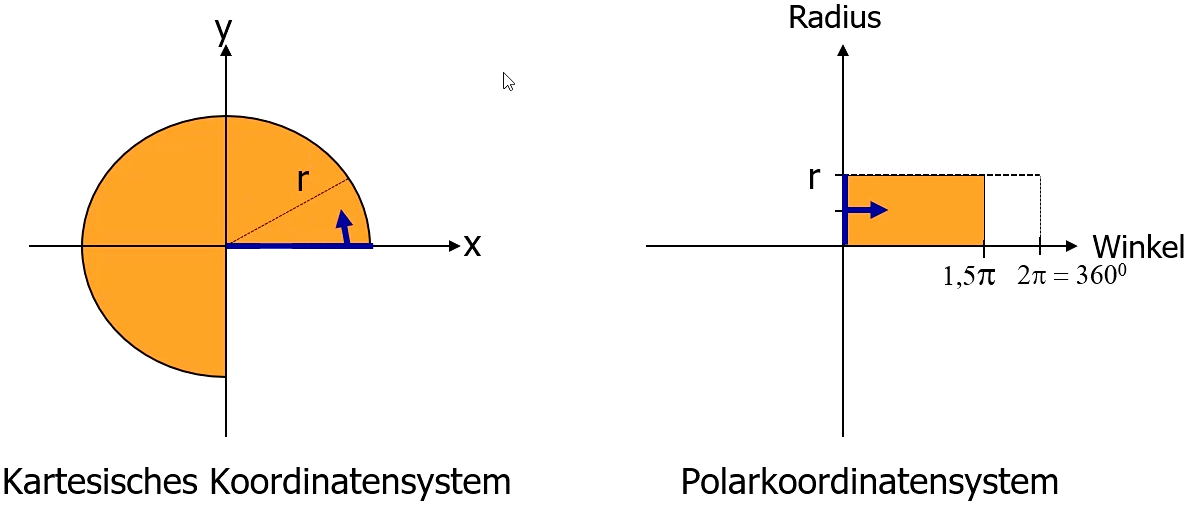
\includegraphics[width=350px]{Polarkoordinatensystem_Kreisausschnitte.png}


\subsection{Zylinderkoordinatensystem}

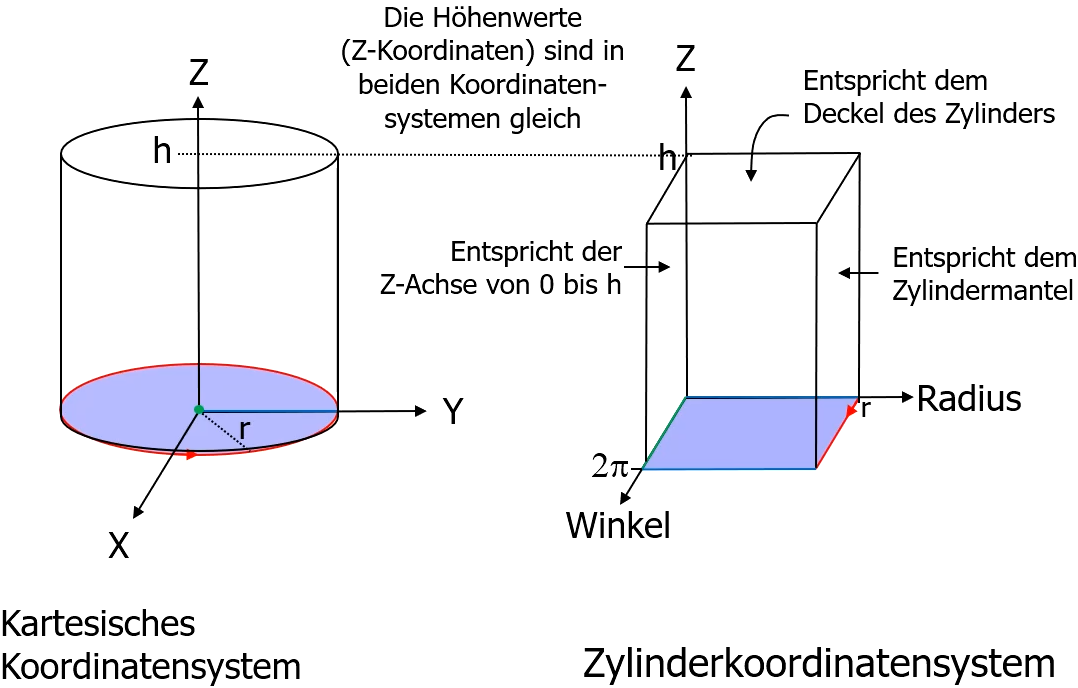
\includegraphics[width=350px]{Zylinderkoordinatensystem.png}

Das Zylinderkoordinatensystem ist ein 3-dimensionales Koordinatensystem, welches das Polarkoordinatensystem durch die z-Achse erweitert. Dabei ist die z-Achse unverändert so, wie sie auch im kartesischen Koordinatensystem ist. Somit ist die Umrechnung zwischen 3-dimensionalem kartesischen Koordinatensystem und Zylinderkoordinatensystem für x- und y-Koordinaten genau wie beim Umrechnen zwischen dem 2-dimensionalen kartesischen Koordinatensystem und dem Polarkoordinatensystem. Die z-Koordinate kann direkt übernommen werden.\\
Hier

\subsection{Kreiskoordinatensystem}

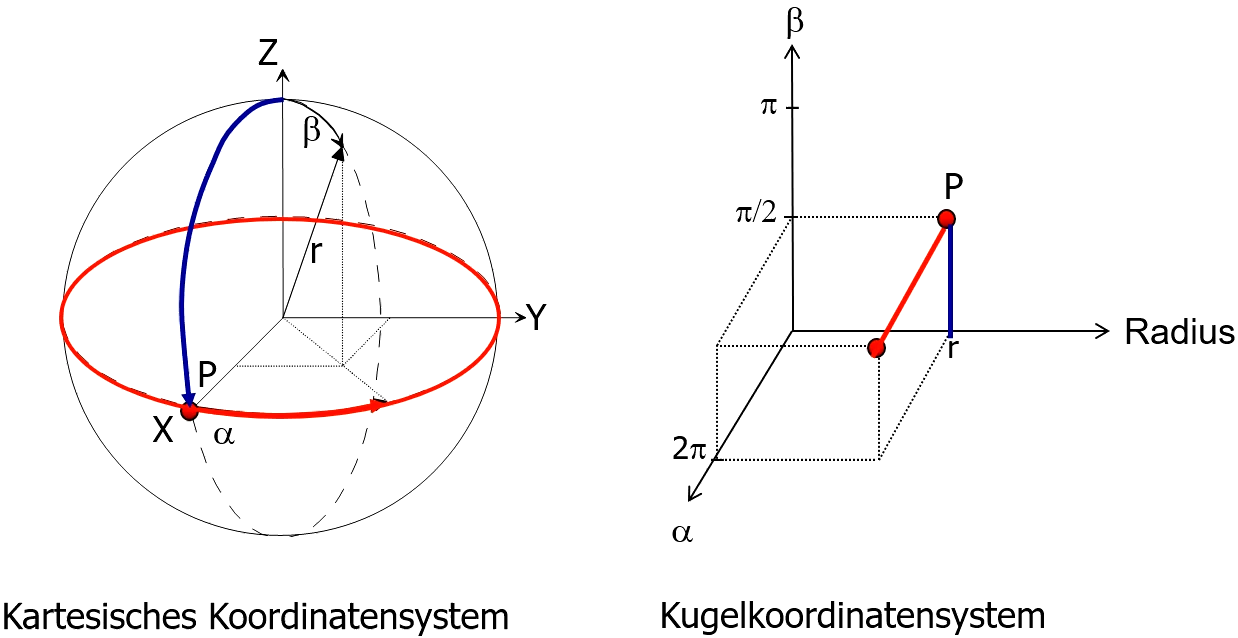
\includegraphics[width=400px]{Kugelkoordinatensystem.png}

Im Kreiskoordinatensystem wird die Position eines Punktes auf einer Kugeloberfläche mittels zweier Winkel $\alpha$ und $\beta$ beschrieben. Durch den Radius, der die Größe der Kugel bestimmt, kann dann jeder Punkt P im Raum beschrieben werden.\\
Einer der beiden Winkel (hier $\alpha$) muss $360°=2\pi$ abdecken. Der andere Winkel (hier $\beta$) muss nur $180°=pi$ abdecken. Denn, wenn wir die Linie, die von $\beta$ Bestimmt wird (hier in \textcolor{blue}{blau}) um den halben Kreis, also bis $\beta = 180°$ ziehen, können wir durch die Rotation um $\alpha = 360°$ (hier in \textcolor{red}{rot}) bereits die gesamte Oberfläche der Kugel abdecken.\\
Hier noch 2 Beispiele:\\
\\
\subsubsection{Äquatorebene im Kugelkoordinatensystem}
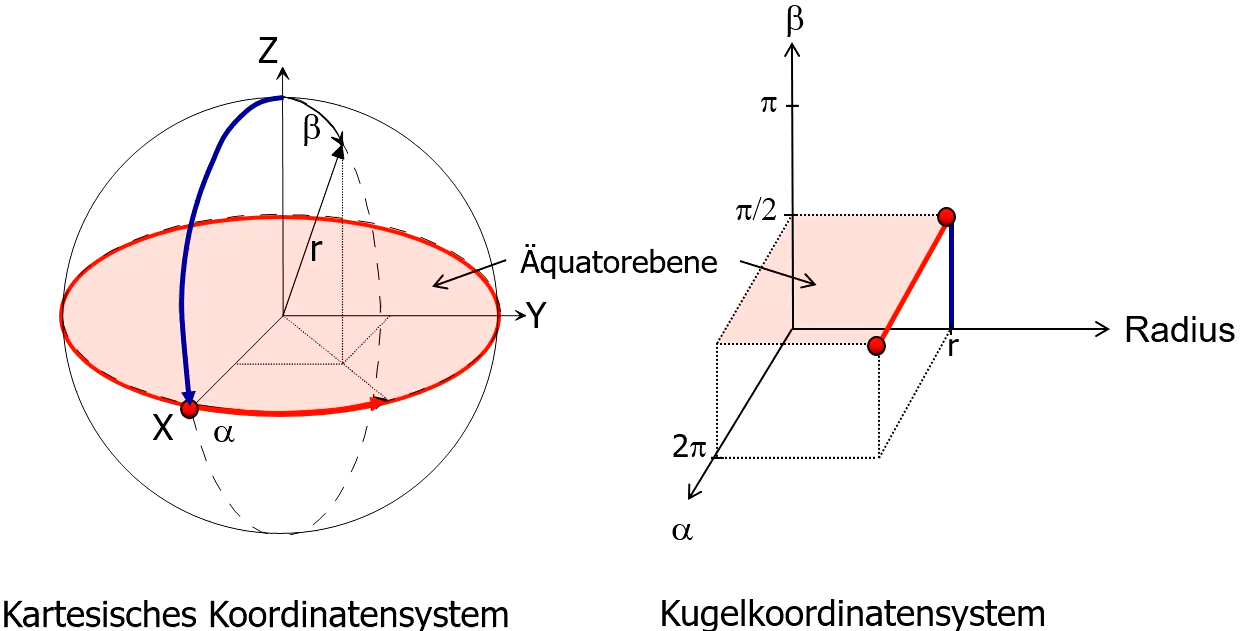
\includegraphics[width=300px]{Kugelkoordinatensystem_Aequatorebene.png}

\subsubsection{Halbkreise im Kugelkoordinatensystem}

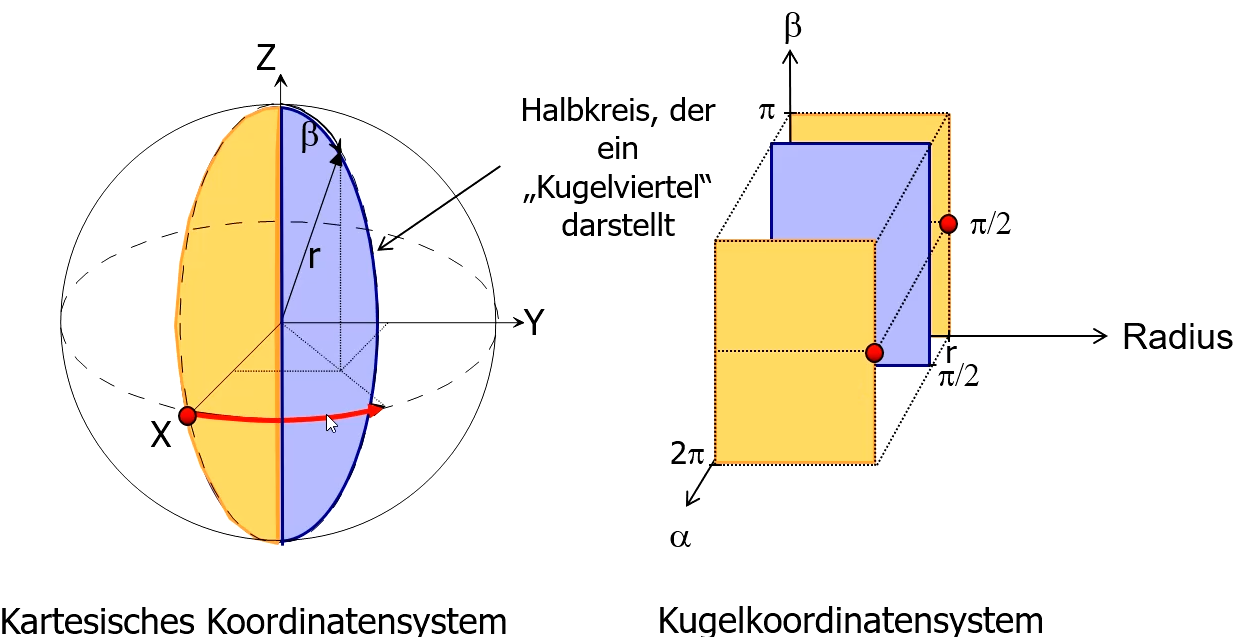
\includegraphics[width=300px]{Kugelkoordinatensystem_Halbkreis.png}

\section{Visualisierungstechniken}
Bei den Visualisierungstechniken beschäftigen wir uns vor Allem damit, wie man die Färbung Pixeln berechnen kann.

\subsection{Lineare Interpolation}

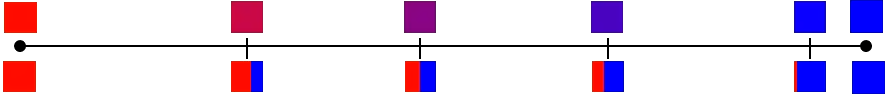
\includegraphics[width=400px]{LineareInterpolation.png}

Die lineare Interpolation beschreibt die Berechnung der Farbe eines Punktes P, der auf einer Linie liegt. Die Linie befindet sich zwischen 2 Punkten \textcolor{red}{A} und \textcolor{blue}{B} für welche die Farbe vorgegeben/bekannt ist. Jedem Punkt auf der Linie wird nun ein Anteil der Farben der Punkte A und B entsprechend seiner relativen Nähe zum jeweiligen Punkt zugeteilt.\\
Die entsprechende Rechnung ist die folgende:\\
\\
$t$ beschreibt das Verhältnis der Länge des Vektors $\overrightarrow{\mathrm{AT}}$ zur Länge des Gesamtvektors $\overrightarrow{\mathrm{AB}}$:\\
$ t = \frac{|\overrightarrow{\mathrm{AT}}|}{|\overrightarrow{\mathrm{AB}}|}$\\
$F(X)$ beschreibt die Farbe eines Punktes $X$.\\
Somit gilt nun für die Farbe des Punktes $P$:\\
\begin{math}
    F(P) = (1 - t) \cdot F(A) + t \cdot F(B)
\end{math}

\subsection{Bilineare Interpolation}

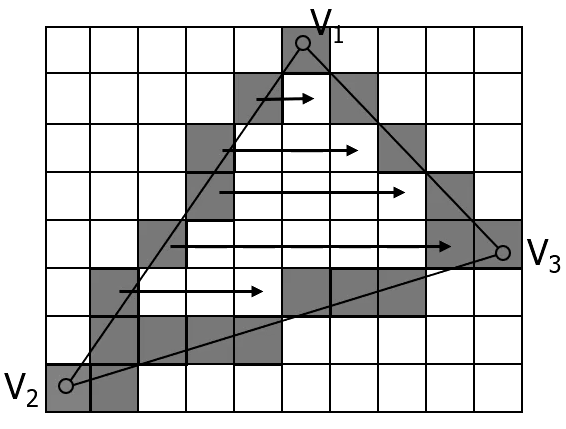
\includegraphics[width=200px]{bilineareInterpolation.png}

Die bilineare Interpolation ist ein Verfahren zur Berechnung von Farbwerten auf Flächen, die durch Eckpunkte mit vorgegebenen Farbwerten definiert werden. Dabei werden zunächst Farbwerte der Kanten durch lineare Interpolation der Eckpunkte berechnet (graue Quadrate). Danach können dann horizontal (prinzipiell könnte man das natürlich auch vertikal machen) die Farbwerte der Pixel jeder Reihe durch lineare Interpolation aus den Kanten berechnet werden (schwarze Pfeile).

\subsection{Visualisierung unter Berücksichtigung von Licht}
\subsubsection{Arten von Lichtquellen}
\textbf{Gerichtete Lichtquelle:}\\
Die Strahlen treffen parallel ein. Entsteht in der Realität annäherungsweise, wenn die Lichtquelle nahezu unendlich weit entfernt ist. Bsp.: Sonne

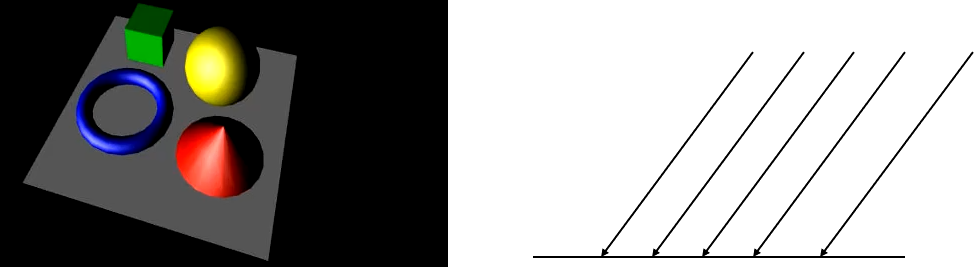
\includegraphics[width=400px]{GerichteteLichtquelle.png}

\vspace{5px}

\textbf{Punktlichtquelle:}\\
Ein Lichtquelle im lokalen Umfeld, die Strahlen in alle Richtungen abgibt. Auf diese Weise treffen Lichtstrahlen an unterschiedlichen Positionen auf einer Ebene mit unterschiedlichen Winkeln auf.

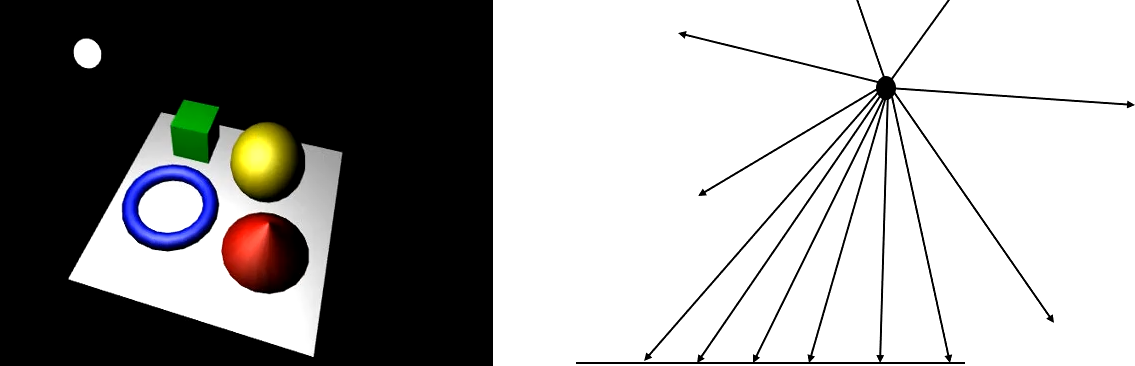
\includegraphics[width=400px]{Punktlichtquelle.png}

\vspace{5px}

\textbf{Spotlight-Lichtquelle:}\\

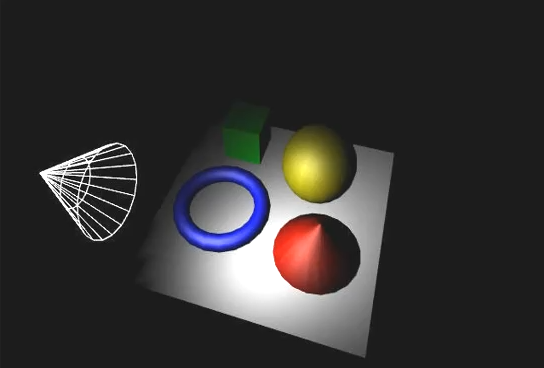
\includegraphics[width=200px]{SpotlightLichtquelle.png}

Die Strahlen kommen bezüglich des Winkels wie bei einer Punktlichtquelle an. Allerdings gibt die Lichtquelle nur in einem bestimmten Radius Licht ab. Die Lichtquelle hat also einen bestimmten Öffnungswinkel. Außerdem wird das Licht schwächer, wenn sich die Lichtquelle weiter entfernt.

\subsubsection{Phong'sches Beleuchtungsmodell}


Das Phong'sche Beleuchtungsmodell ist ein Modell, das zur Berechnung der Beleuchtung von Objekten benutzt werden kann. Dabei wird zunächst angenommen, dass die Lichtquelle Punktförmig ist. Dann werden 3 Beleuchtungsarten benutzt, deren Summe dann ein halbwegs realistisches Bild ergeben sollen:
\begin{itemize}
    \item Die \textbf{Spiegelnde Reflexion} bezeichnet die Reflexion, bei welcher der Einfallswinkel auf die Oberfläche, sowie die Position des Betrachters entscheidend sind. Hierbei entstehen bei richtigem glänzende Flächen, andernfalls bleibt die Oberfläche schwarz, da kein Licht zum Betrachter gelangt. Diese Art von Reflexion kennen wir von Spiegeln oder hochglanzpolierten Oberflächen. Das reflektierte Licht hat die hier die Farbe der der Lichtquelle.
    \item Die \textbf{Diffuse Reflexion} bezeichnet die Art von Reflexion, die man von Matten Oberflächen kennt. Dabei wird das Licht in alle Richtungen gleichermaßen reflektiert. Die diffuse Reflexion ist somit unabhängig vom Standpunkt des Betrachters. Sie ist aber abhängig vom Einfallswinkel des Lichts. Dieser bestimmt nämlich die Helligkeit der Reflexion. Das reflektierte Licht hat die hier die Farbe der Oberfläche.
    \item Die \textbf{Ambiente Reflexion} bezeichnet die Art von Reflexion, die durch eine Grundbeleuchtung der Umgebung entsteht. Die Grundbeleuchtung ist für die gesamte Szene gleich und von der Lichtquelle und dem Betrachter unabhängig. Diese Reflexion soll modellieren, dass durch wiederholte Reflexion von Licht an der Umgebung schließlich die gesamte Umgebung eine Gewisse Helligkeit hat. Dies kennt man, wenn es in einem dunklen Raum nie ganz dunkel wird, da immernoch Licht von Lichtquellen in den Raum gelangen kann, die nicht in der Szene bekannt sind. Das reflektierte Licht hat die hier die Farbe der Oberfläche.
\end{itemize}

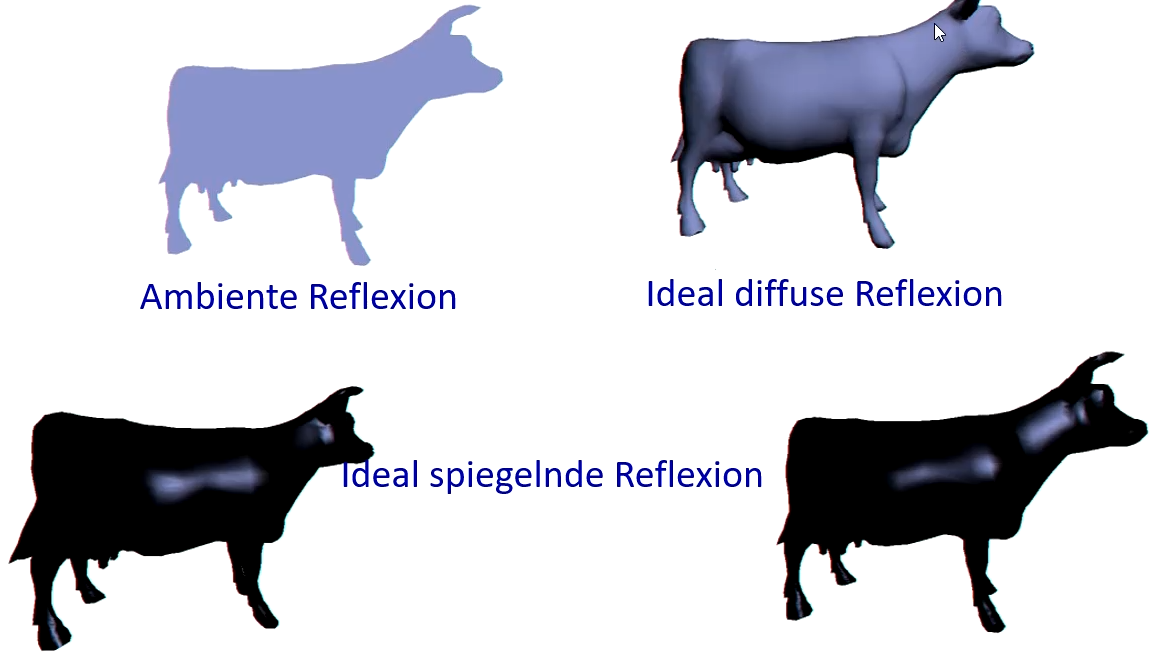
\includegraphics[width=300px]{PhongschesReflexionsmodell.png}

\subsubsection{Beleuchtungsberechnung - Methoden}
Bei der Berechnung der Beleuchtung nach dem Phong'schen sind die Winkel nötig, in denen das Licht auf die Oberfläche trifft (benötigt für spiegelnde und diffuse Reflexion). Um den Winkel berechnen zu können ist ein Normalenvektor für den Punkt/die Fläche nötig.

\vspace{10px}
\textbf{Flat Shading - Mittels Flächennormalen:}\\

\includegraphics[height=130px]{Beleuchtungsberechnung-Flächennormale-vector.png}
\hspace{15px}
\includegraphics[height=130px]{Beleuchtungsberechnung-Flächennormale.png}

Für jede Fläche wird ein Normalenvektor bestimmt. Somit wird auch für jede Fläche genau ein Eintrittswinkel und somit ein Farbwert bestimmt. Um mit dieser Berechnungsmethode ein realistisches Bild zu erschaffen benötigt man sehr viele einzelne Flächen.

\vspace{10px}
\textbf{Gouraud Shading - Mittels Eckennormalen}\\

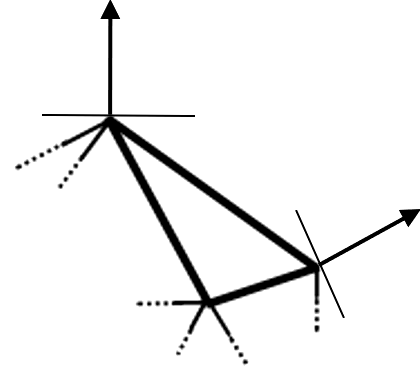
\includegraphics[height=130px]{Beleuchtungberechnung-Eckennormale-vector.png}
\hspace{150px}
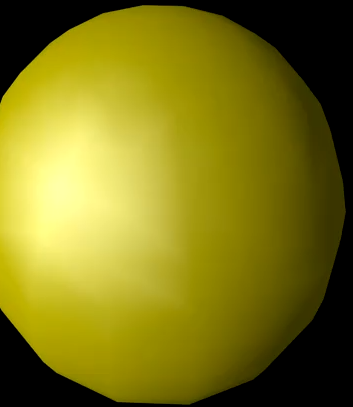
\includegraphics[height=130px]{Beleuchtungberechnung-Eckennormale.png}

Es wird ein Normalenvektor für jeden Eckpunkt der Oberfläche bestimmt. die Farbwerte der Flächen berechnen sich dann durch bilineare Interpolation der Eckpunkte. Mit dieser Methode kann recht einfach und performant ein Bild sehr realistisch Aussehen. Das Objekt selbst sieht glatt aus, Obwohl die Oberfläche aus wenigen Teilflächen besteht (Einsparung von Speicherplatz gegenüber der Benutzung von Flächennormalen mit hoher Anzahl an Flächen).\\

\begin{wrapfigure}{r}{0.35\textwidth}
    \centering
    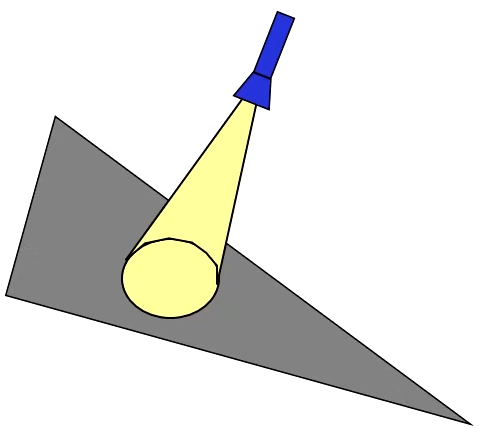
\includegraphics[height=100px]{GrenzenDesGouraudShading.png}
\end{wrapfigure}

Die \textbf{Grenze des Gouraud Shading}s ist, dass es bei sehr großen Flächen und sehr nahen Lichtquellen oder Spotlight-Lichtquellen dazu führen kann, dass die realen Farbwerte in der Mitte so verschieden zu den Farbwerten der Eckpunkte sind, dass die Fläche eine falsche Farbe erhält. Im unteren Beispiel würde so die Fläche nicht beleuchtet gerendered werden, weil ihre Eckpunkte nicht beleuchtet werden.

\vspace{10px}
\newpage
\textbf{Phong Shading - Berechnung jedes Pixels}\\
Beim Phong Shading wird für jeden Darzustellenden Pixel ein eigener Normalenvektor berechnet. Damit kann dann der Farbwert für diesen Pixel genau bestimmt werden. Mit diesem Verfahren können uns nun keine Dinge mehr entgehen, so wie es beim Gouraud Shading der Fall war. Allerdings ist die Berechnungszeit dementsprechend auch länger. Die Leistung der heutigen CPUs und GPUs hat aber dazu geführt, dass dieser Nachteil nicht mehr relevant ist.
\section{Digitale Bilder}

\subsection{Darstellung mittels Pixel}
\label{sec:pixel}
Rastergraphiken, die wir nun betrachten wollen, werden als Matrix einzelner Farbpunkte dargestellt, die man Pixel nennt. Dadurch, dass jedes Pixel einen gewissen Farbwert hat, entsteht dann ein komplexes Bild. Pixel können auf 2 verschiedene Arten betrachtet werden:

\subsubsection*{Geometrische Betrachtung}

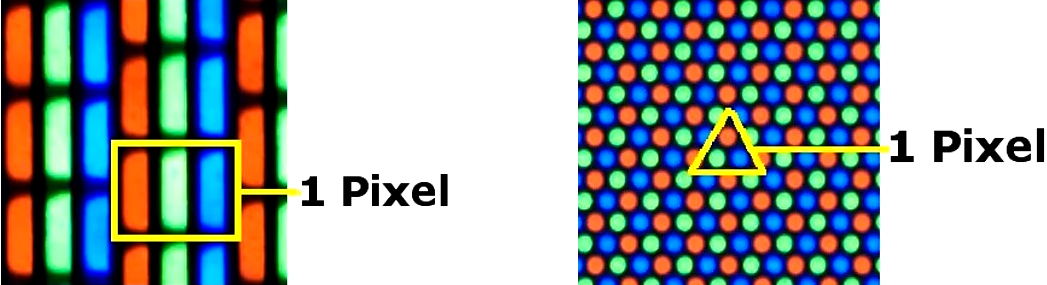
\includegraphics[height=80px]{Pixel_Hardware.png}

Ein Pixel ist i.d.R kein atomarer Baustein eines Hardwaregeräts. Stattdessen besteht er aus i.d.R. 3 Lichtern, welche die 3 Grundfarben ausstrahlen. Wiese das so ist werden wir noch in einem der folgenden Kapitel erfahren, wenn es um Farbmodelle geht.\\
Bei der geometrischen Betrachtung interessieren wir uns für die Form und Anordnung der Bestandteile eines einzelnen Pixels, sowie der Pixel zueinander.

\subsubsection*{Photometrische Betrachtung}
Die Photometrische Betrachtung bezieht sich auf die Darstellung von Objekten mit Farben/Grautönen. Es geht also darum welchen Wert die Pixel annehmen sollen. Dies ist die Betrachtung, die uns im Folgenden beschäftigen wird.

\subsection{Optische Wahrnehmung}
\subsubsection*{Physikalische und Biologische Aspekte}

\begin{wrapfigure}{r}{0.5\textwidth}
    \centering
    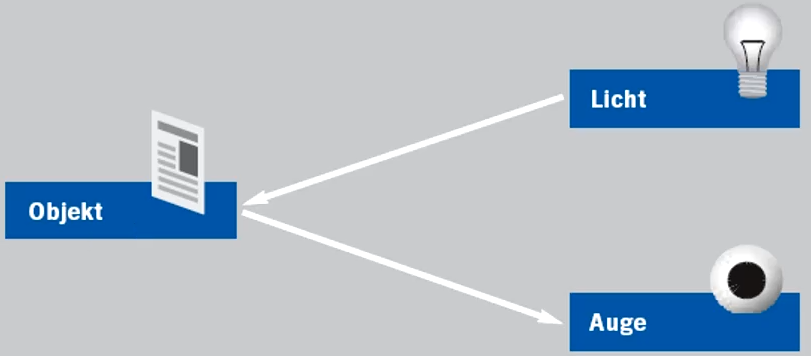
\includegraphics[height=100px]{OptischeWahrnehmung_Reflexion.png}
    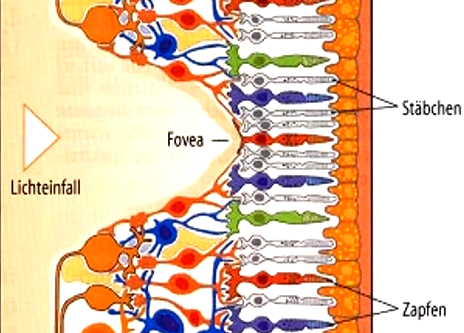
\includegraphics[width=200px]{OptischeWahrnehmung_Retina.png}
\end{wrapfigure}

Objekte werden sichtbar, indem Licht auf sie fällt, reflektiert wird und in unser Auge gelangt. Je nach Oberfläche und Material des Objektes werden unterschiedliche Wellenlängen und damit Farben des Lichtes mehr oder weniger reflektiert. Die nicht reflektierten Lichtstrahlen werden absorbiert und somit in Wärmeenergie umgewandelt.\\

Auf der Retina (syn. Netzhaut) befinden sich Sinneszellen, die Stäbchen und Zapfen. Die Stäbchen sind für das Helligkeitssehen verantwortlich. Die Zapfen gibt es in den 3 Ausprägungen rot, grün und blau. Die Zapfen reagieren hauptsächlich auf die Wellenlänge von licht ihres Typs.\\
Die Empfindlichkeit für Helligkeit ist wesentlich Stärker als die für Farben. Somit können bei wenig Licht fast nur noch die Stäbchen aktiviert werden und wir sehen Nachts bloß schwarz-weiß. Das wird nocheinmal interessant, wenn es um das HSV-Farbmodell geht.

\subsubsection*{Subjektivität der optischen Wahrnehmung}

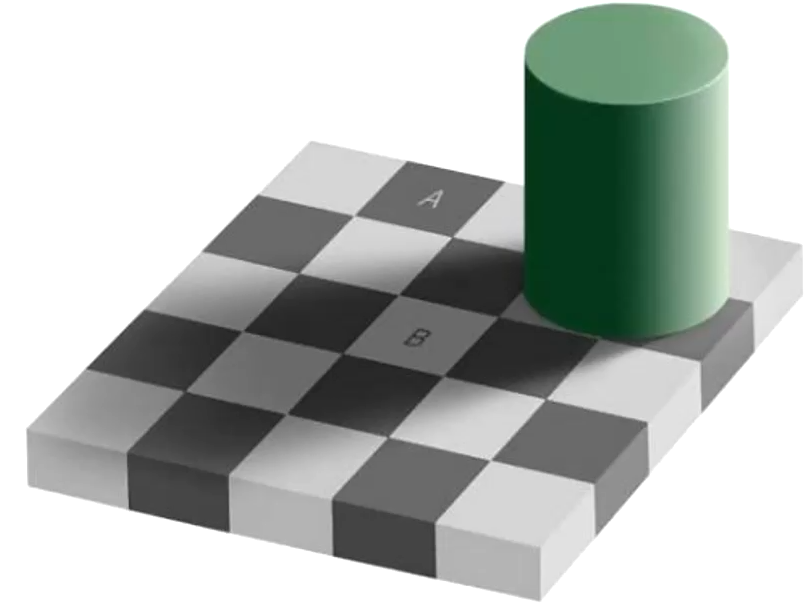
\includegraphics[height=100px]{OptischeWahrnehmung_taeuschungen.png}

Die optische Wahrnehmung ist stark Subjektiv und keinesfalls absolut. Sie wird vor allem durch Erfahrungswerte und neurologische Effekte beeinflusst.\\
Im oberen Beispiel sieht das Feld A viel dunkler aus als das Feld B. Das Gehirn erkennt, dass das Feld B im Schatten liegt und hellt daher seine Farbe auf. Es erkennt auch das Muster des Schachbretts und versucht die Farben so zu interpretieren, dass das Muster nicht gebrochen wird.

\subsection{Farbmodelle}

\subsubsection{CIE Farbraum}
Der CIE Farbraum ist die erste Standardisierung eines Farbraums. Er umfasst alle vom Menschen wahrnehmbaren Farben. Die folgenden Farbmodelle basieren auf diesem Farbraum.

\subsubsection{Hardwareorientiertes Modell - RGB}
\label{sec:RGB}

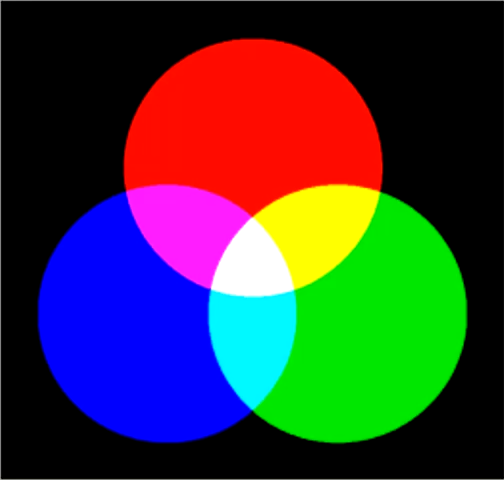
\includegraphics[height=150px]{RGB_circles.png}
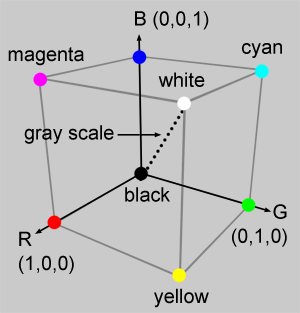
\includegraphics[height=150px]{RGB_cube.png}

Beim RGB Farbmodell besteht jede Farbe aus einer Mischung der 3 Grundfarben \textcolor{red}{rot}, \textcolor{green}{grün} und \textcolor{blue}{blau}. Das bedeutet, dass für jeden Pixel ein Vektor $\vec{v} = \left(\begin{smallmatrix}r \\ g \\ b \end{smallmatrix}\right)$ mit 3 Werten definiert wird.\\
Das RGB Modell ist ein additives Farbmodell. Das bedeutet, dass die Menge an Licht sich bei steigendem Wert einer Komponente des Farbvektors erhöht. Das bedeutet, dass $\vec{v_1} = \left(\begin{smallmatrix}0 \\ 0 \\ 0 \end{smallmatrix}\right)$ schwarz entspricht und ${v_2} = \left(\begin{smallmatrix}1 \\ 1 \\ 1 \end{smallmatrix}\right)$ weiß entspricht.\\
Das additive Farbdenken kennen wir, wenn wir mit Lampen, die verschiedene Farben haben, auf eine weiße Wand leuchten (1. Bild). Das weiße Licht entsteht bei Anwesenheit aller Farben. Entspricht dieses Farbmodell ziemlich direkt der Ansteuerung der einzelnen \hyperref[sec:pixel]{Pixelkomponenten, die wir schon kennengelernt haben}.\\
Die Gerade, die von schwarz nach weiß führt nennt man Unbuntgerade und enthält alle Grautöne. Für Grautöne gilt, dass R=G=B. Das Sechseck, dass aus $\overline{bm}$, $\overline{mR}$, $\overline{Ry}$, $\overline{yG}$, $\overline{Gc}$ und $\overline{cB}$ gebildet wird, enthält alle maximal gesättigten Farben, d.h. Farben mit Sättigung = 100\% \slash 255. Je höher der grauanteil ist (i.e. näher an der Unbuntgerade), desto weniger gesättigt ist die Farbe.\\
\\
In einer Erweiterung des RGB-Modells, dem RGBA-Modell, wird ein weiterer sogenannter Channel angefügt, der sich Alpha-Channel nennt und die Sichtbarkeit bzw. Transparent darstellt. Da wir jeden Channel mit einer genauigkeit von 8Bit darstellen, benötigt RGBA dann 4Byte pro Pixel.

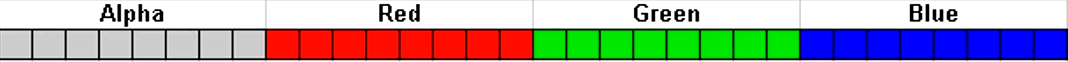
\includegraphics[width=300px]{RGBA.png}

\subsubsection{Hardwareorientertes Modell - CMY}

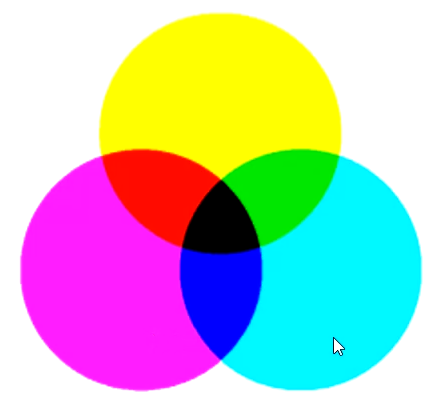
\includegraphics[height=150px]{CMY_circles.png}
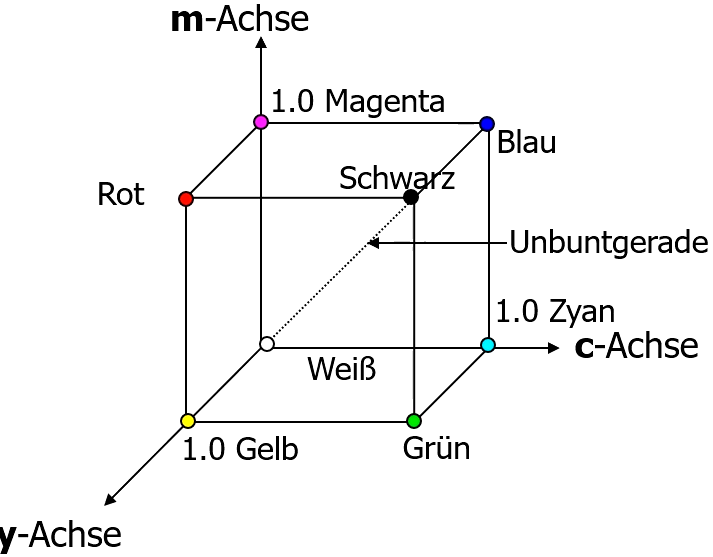
\includegraphics[height=150px]{CMY-cube.png}

Das CMY (Cyan Magenta Yellow) Modell ist ein subtraktives Farbmodell mit den entsprechenden Grundfarben. Umso höher die Werte der Komponenten sind, desto dunkler wird die Farbe, es trifft also weniger Licht ins Auge (subtraktiv). Wir kennen dieses Prinzip beim Mischen von Wasserfarben.\\
Der Farbwürfel des CMY-Modells entsteht aus dem Farbwürfel des RGB-Modells, indem man die Achsenbeschriftung ändert und den Würfel so dreht, dass seine Weiße Ecke im Ursprung liegt.\\
Während das RGB der Lichtmischung entspricht und damit für Displays verwendet werden kann, kann das CMY Modell für Pigmentmischung z.B. beim Drucken verwendet werden.\\
Das \textbf{CMYK} (CMY Blac\textbf{k}) Modell ergänzt das CMY-Modell um einen weiteren Anteil an Schwarz. Der Vorteil dieses Modells ist die bessere Darstellung von Schwaztönen und Konturen z.B. beim Drucken. Eigentlich ist der Black-Channel redundant, da ${v_{CMY}} = \left(\begin{smallmatrix}1 \\ 1 \\ 1 \end{smallmatrix}\right)$ bereits schwarz entspricht. In der Praxis sind die Farben aber nicht perfekt rein, sodass beim Mischen kein perfektes Schwarz entsteht.

\subsubsection{Wahrnehmungorientiertes Modell - HSV}

\begin{wrapfigure}{r}{0.5\textwidth}
    \centering
    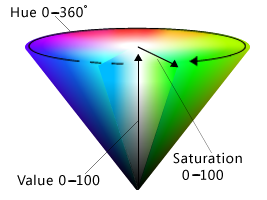
\includegraphics[height=150px]{HSV_room.png}
\end{wrapfigure}

Beim HSV Modell wird eine Farbe in einem Zylinderkoordinatensystem mit den Werten \textbf{H}ue=Farbton (Winkel des Kreisausschnitts 0-365° bzw. 0\% - 100\%), \textbf{S}aturation = Sättigung (Radius des Kreises) und \textbf{V}alue = Helligkeit/Intensität (vertikale Achse) dargestellt. Der Farbverlauf des oberen Randes des Farbkegels entspricht genau dem Sechseck der maximal gesättigten Farben des \hyperref[sec:RGB]{RGB-Würfels}.\\
Im folgenden sehen wir ein Beispiel für die Zerlegung eines Farbbilds in die 3 HSV Kanäle, wobei jeder extrahierte Wert $x \in [0, 1]$ wieder als Wert eines schwarz-weiß Bildes interpretiert wird, wobei 0 schwarz entspricht und 1 weiß.\\
Die Bilder sind in der Reihenfolge All, \textbf{S}aturation, \textbf{V}alue, \textbf{Hue} gezeigt:

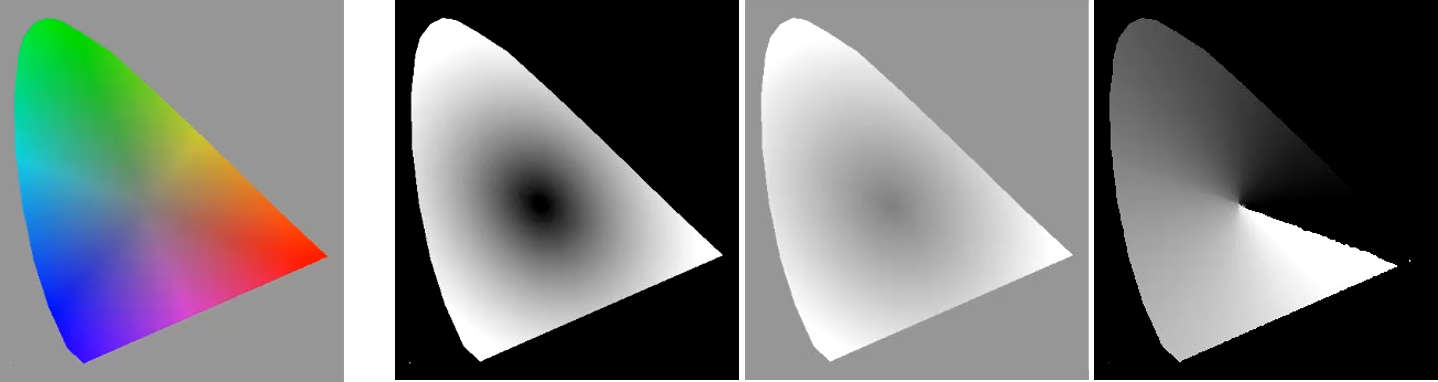
\includegraphics[height=100px]{HSV_decomposition.png}

\textbf{Erklärung der Zuordung:}\\
Auf dem \textbf{ersten Bild} ist der graue Hintergrund schwarz, da die Sättigung von Grautönen Null ist. Außerdem ist die Außenkante des Objektes weiß, da hier die maximal gesättigten Farben liegen. Somit handelt es sich um die Saturation.\\
Auf dem \textbf{zweiten Bild} ist der Hintergrund identisch mit dem grauen Hintergrund vom Originalbild, denn Ein Grauton entspricht in HSV einem puren Helligkeitswert. Somit handelt es sich um Value.\\
Auf dem \textbf{dritten Bild} ist der Hintergrund schwarz, da Grautöne in HSV keinen Farbwert haben. Außerdem zeigt sich der Farbverlauf als lineare Steigerung der Graustufen, da die Farben genau so angeordnet sind, wie sie im HSV-Farbkegel angeordnet sind. Somit steigt der Wert des ihnen zugeordneten Winkels stetig.\\
\\
Da das HSV-Modell die Farben getrennt von der Helligkeit speichert, konnte mithilfe dieses Modells früher (in der Zeit des Schwarz-Weiß-Fernsehens) einfach ohne Rechnen aus einem Farbfilm ein Schwar-Weiß-Film extrahiert werden, der an private Haushalte ausgestrahlt werden konnte.\\
Außerdem können manche Algorithmen der Bildverarbeitung schneller mit solchen Bildern arbeiten, da viele Techniken hauptsächlich auf Helligkeitswerten basieren.

\subsubsection{YUV Farbmodell und 4:1:1 Farbraum}

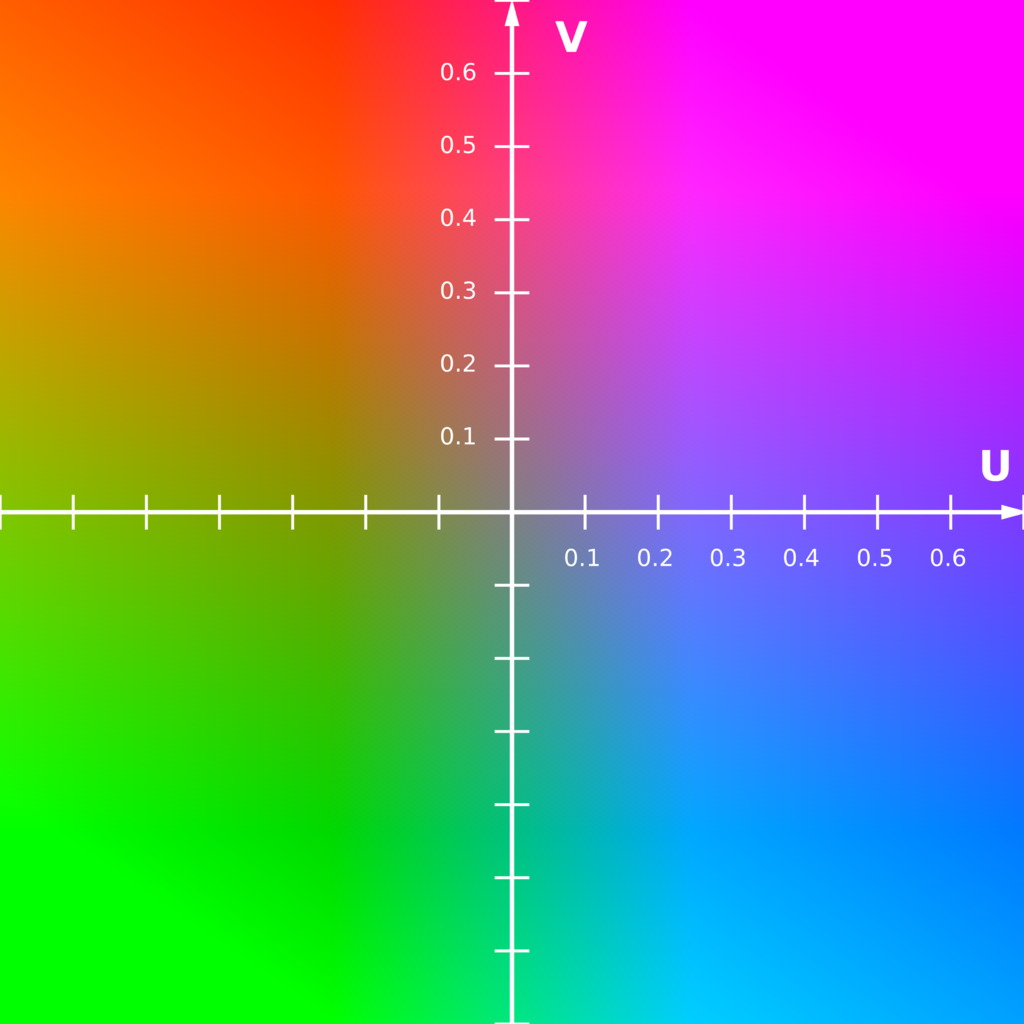
\includegraphics[height=150px]{YUV.png}

Im YUV-Farbmodell wird eine Farbe mittels eines Chrominanz-Wertes, der aus 2 sättigungslosen Farben U und V (siehe Bild) besteht, und einem Luminanzwert (Helligkeit) bestimmt.\\
Dieses Modell kann benutzt werden, um Bilder zu komprimieren. Denn das menschliche Auge ist sehr viel empfindlicher für Helligkeit als für Farbe. Somit kann man, wenn die Farbe und Helligkeit getrennt gespeichert sind, weniger Daten für die Farbe als für die Helligkeit benutzen, ohne dass es für dem Menschen wahrnehmbar ist. Oft wird der sog. 4:1:1 Farbraum verwendet, in dem für 4 Pixel auch 4 Helligkeitswerte gespeichert werden, aber nur 1 Farbwert U und ein Farbwert V.
\section{Bildverarbeitung}
\subsection{Maße zur Beurteilung von Bildern}


\subsubsection{Histogramme}
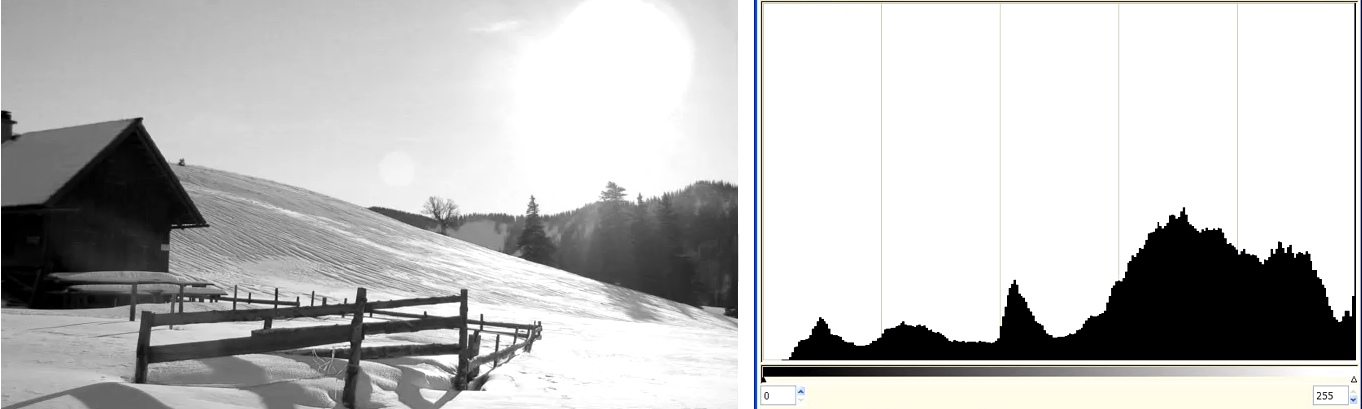
\includegraphics[height=150px]{Histogramm1.png}

Mit Histogrammen stellen wir die Häufigkeitsverteilung von Werten von Pixeln in einem Bild dar. Da wir mit 8 Bit Wertebereicht [0, 255] arbeiten, gibt es 256 Werte denen eine absolute Häufigkeit im Bereich [0, n] zugeordnet wird, wobei n die Anzahl der Pixel des Bildes ist.\\
Aus diesen Histogrammen kann man Informationen über das Bild extrahieren. Beispielsweise kann man im oberen Beispiel anhand des Histogramms sehen, dass der Großteil der Pixel einen hohen Wert hat, also das Bild eher hell ist. Des Weiteren können wir folgende Dinge erkennen:
\begin{itemize}
    \item \textbf{Belichtungsfehler:}\\
          Belichtungsfehler kann man daran erkennen, dass in einem Bild das eine Ende des Wertebereichs ungenutzt bleibt, am anderen Ende aber Häufungen auftreten (wie im oberen Beispiel)
    \item \textbf{Kontrast:}\\
          Der Kontrast bezeichnet die Differenz zwischen dem minimalen und maximalen genutzten Grauwert. Ein maximaler Kontrast nutzt den vollen Wertebereich. Das bedeutet bei 8 bit Bildern, dass es jeweils mindestens ein Pixel mit den Werten 0 und 255 im Bild geben muss. ein kleiner Kontrast entsteht, wenn alle genutzten Werte nah beieinander liegen, bis hin zum minimalen Kontrast, bei dem jedes Pixel den gleichen Wert hat.
    \item \textbf{Dynamik:}\\
          Die Dynamik beschreibt wie hoch der Anteil der genutzten Werte im Bereich zwischen dem minimalen und maximalen genutzten Wert liegt. Das bedeutet, dass eine minimale Dynamik entsteht, wenn es nur Pixel mit den Werten 0 und 255 gibt. Dann ist nämlich der genutzte Wertebereich maximal, nämlich [0, 255], und die Anzahl der genutzten Werte dieses Bereichs minimal, nämlich 2. Eine maximale Dynamik entsteht dann, wenn alle Werte zwischen dem höchsten und niedrigsten genutzten Wert genutzt werden. Das obere Bild zeigt z.B. eine maximale Dynamik, da im Wertebereich [20, 255] alle Werte mindestens 1 mal vorkommen und es keine Werte außerhalb dieses Bereichs gibt, die genutzt werden.
\end{itemize}

\subsubsection{Entropie}
Die Entropie einer Nachricht (hier eines Bildes) ist ihr mittlerer Informationsgehalt.
Es gilt: Je mehr Pixel es mit dem gleichen Wert gibt, desto geringer ist der Informationsgehalt dieser Pixel. Das bedeutet, dass die Entropie zunimmt, wenn sich die Verteilung der Grauwerte eines Bilds einer Gleichverteilung mit vollem Kontrast annähert. Auf die mathematische Berechnung wollen wir an dieser Stelle verzichten.

\subsection{Punktoperationen \& lineare Transformationen}
\label{sec:Punktoperationen}
Punktoperationen bezeichnen eine Art von Transformationen bei denen auf jedes Pixel eines Bildes eine Funktion angewendet wird, um das Pixel des Abbilds zu erzeugen, die \textbf{unabhängig von den anderen Pixeln ist}. Das bedeutet, dass die Eingangsvariable der Wert genau eines Pixel ist und die Ausgangsgröße genau der Wert des gleichen Pixels im Abbild. Die Operation wird dann für alle Pixel des Bildes durchgeführt.\\
Die Punktoperationen, die wir betrachten, sind \textbf{lineare Operationen} deshalb nennt man sie auch \textbf{lineare Grauwerttransformationen}. Das bedeutet, dass die Zuordnung eines Wertes eines Pixels im Originalbild zum Pixel im Abbild durch eine lineare Funktion beschrieben wird. Diese Funktion ordnet jedem Wert des farblichen Wertebereichs [0, 255] wieder einen Wert genau dieses Bereichs zu. Die Funktionsgraphen in denen wir das Aufzeichnen nennen wir auch gg\'-Diagramme. Im Grunde ist es eine einfache lineare Funktion. Jedoch können wir auf der x-Achse eine konkrete Verteilung (also ein Histogramm) einzeichnen, und dann die Verteilung dort auf der y-Achse einzeichnen, wo die Säulen der x-Achse auf den Funktionsgraphen treffen würden. So erkennen wir beispielsweise, dass ein Histogramm bei einer Steigung $0 < m < 1$ gestaucht wird (also der Kontrast verringert wird) und für $m > 1$ das Histogramm gestreckt wird (also der Kontrast vergrößert wird). Im unteren Beispiel ist unsere Funktion $g' = g$, die also das Bild auf sich selbst abbildet.\\

Dabei ist unbedingt zu beachten, dass der Funktionsgraph eine ganz normale lineare Funktion ist, die auch ohne das Histogramm dargestellt werden kann. Die Funktion ordnet jedem Farbwert (x-Wert) einen neuen Ergebniswert (y-Wert) zu. Das Histogramm ist nur eine Veranschaulichung der konkreten Anwendung für mehrere Punkte. Wir setzen also den Grauwert jedes Pixels einzeln in die Funktion ein, um seinen Ergebnispixel zu erhalten. Das Histogramm zeigt uns für ein konkretes Bild wie oft welcher x-Wert eingesetzt werden wird.

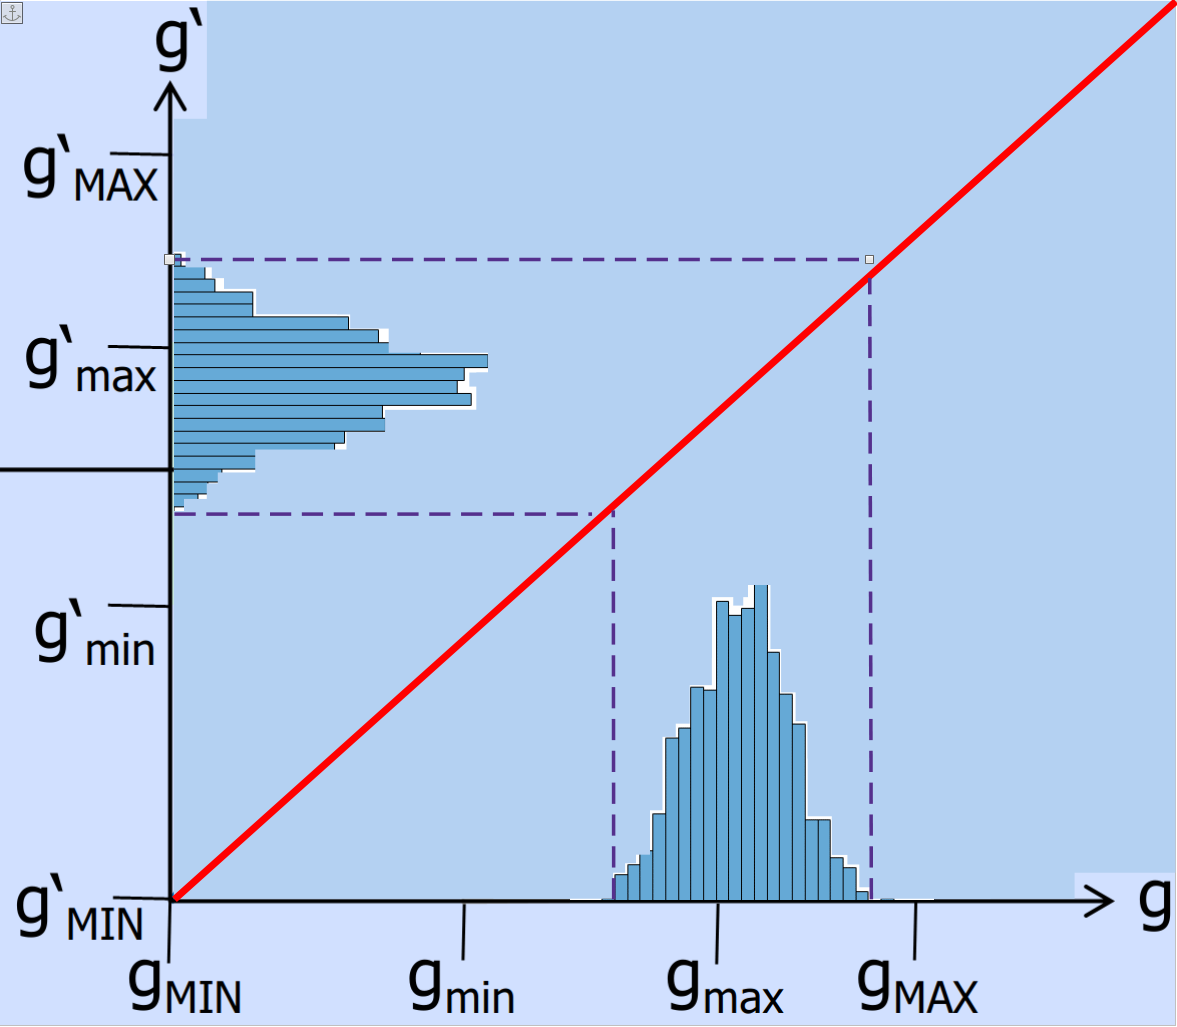
\includegraphics[height=200px]{ggstrichDiagramm.png}

Bei der Wahl der Funktion für die lineare Grauwerttransformation müssen wir darauf achten, dass wir den Wertebereich der Funktion einschränken. Der Definitionsbereich und der Wertebereich müssen meist beide innerhalb unseres Bereichs von Farbwerten, also [0, 255], liegen, damit das Ergebnis wieder ein gültiges Bild ist. Um dies umzusetzen können wir Mathematisch beispielsweise eine min bzw. max Funktion benutzen. Programmiertechnisch gibt es natürlich noch viele andere Wege dieses recht einfache problem zu lösen.\\
Es kann jedoch auch Anwendungsfälle geben, in denen der Definitionsbereich oder Wertebereich nicht [0, 255] sein müssen. Bei den \hyperref[sec:difference-operator]{Differenzoperatoren} werden wir beispielsweise sehen, dass wir die lineare Grauwerttransformation anwenden, um Ergebniswerte wieder in den gültigen Bereich zu bewegen. In diesem Fall können die Eingangswerte z.B. auch negativ sein.
Im folgenden sollen einige Punktoperationen beispielhaft gezeigt werden:\\

\subsubsection{Addition}

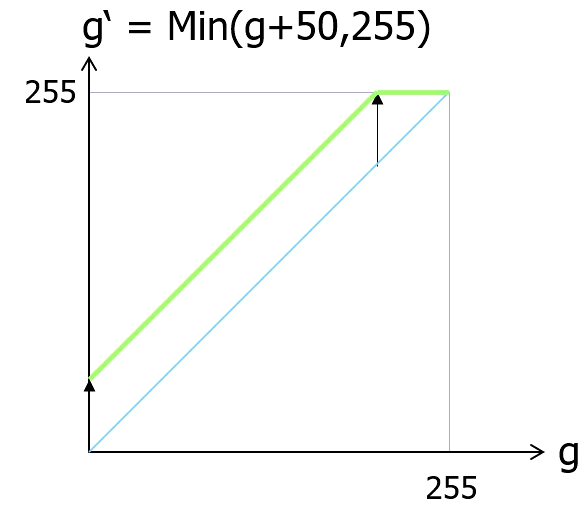
\includegraphics[height=150px]{PunktoperationAddition.png}

Bei dieser Addition wird auf jeden Pixelwert 50 addiert. Das interessante daran ist, dass der Wertebereich [0, 49] des Ergebnisbildes auf jeden Fall ungenutzt bleibt. Außerdem werden alle Säulen des Histogramms von [205, 255] auf den Wert 255 abgebildet. Dadurch entsteht, falls der Bereich [205, 255] überhaupt im Originalbild genutzt wurde, eine erhöhte Häufigkeit für den Pixelwert 255 im Ergebnisbild. Ansonsten sind im Ergebnishistogramm bloß alle Werte um 50 nach rechts verschoben. Logisch gesehen beschreibt die Addition mit einem positiven Wert eine gleichmäßige Aufhellung des Bildes.

\subsubsection{Biniarisierung}
\label{sec:biniarisierung}

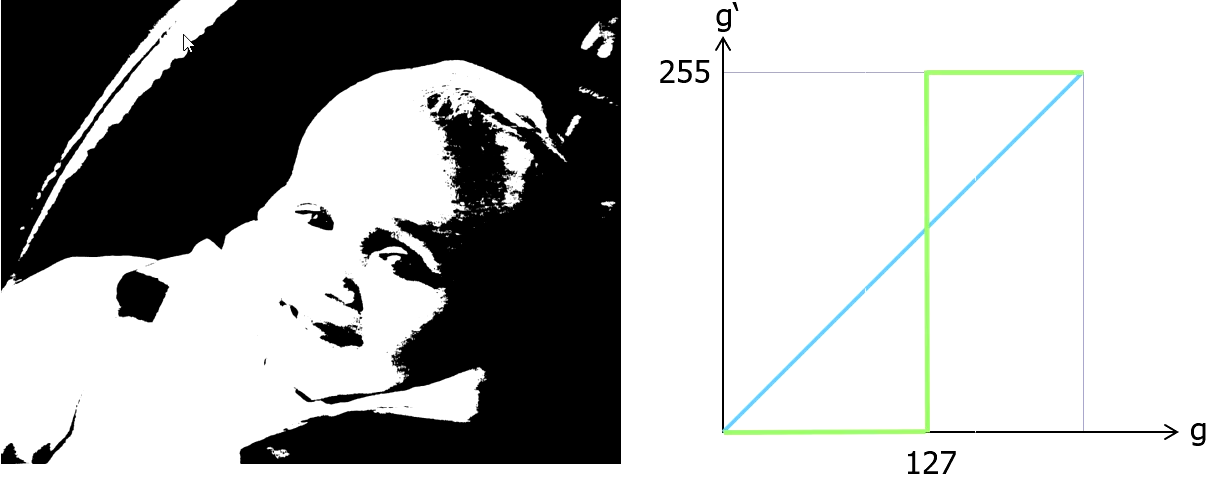
\includegraphics[height=150px]{PunktoperationBiniarisierung.png}

Die Biniarisierung ist eine lineare Grauwerttransformation, bei der die Mächtigkeit des Wertebereichs 2 ist $|W| = 2$. Dabei kann gewählt werden bei welchem Schwellwert der Umbruch vom einen Wert auf den anderen erfolgt (im Beispiel 127) und auf welche 2 Werte abgebildet wird (im Beispiel auf die Werte 0 und 255).

\subsubsection{Äquidensitenbilder}

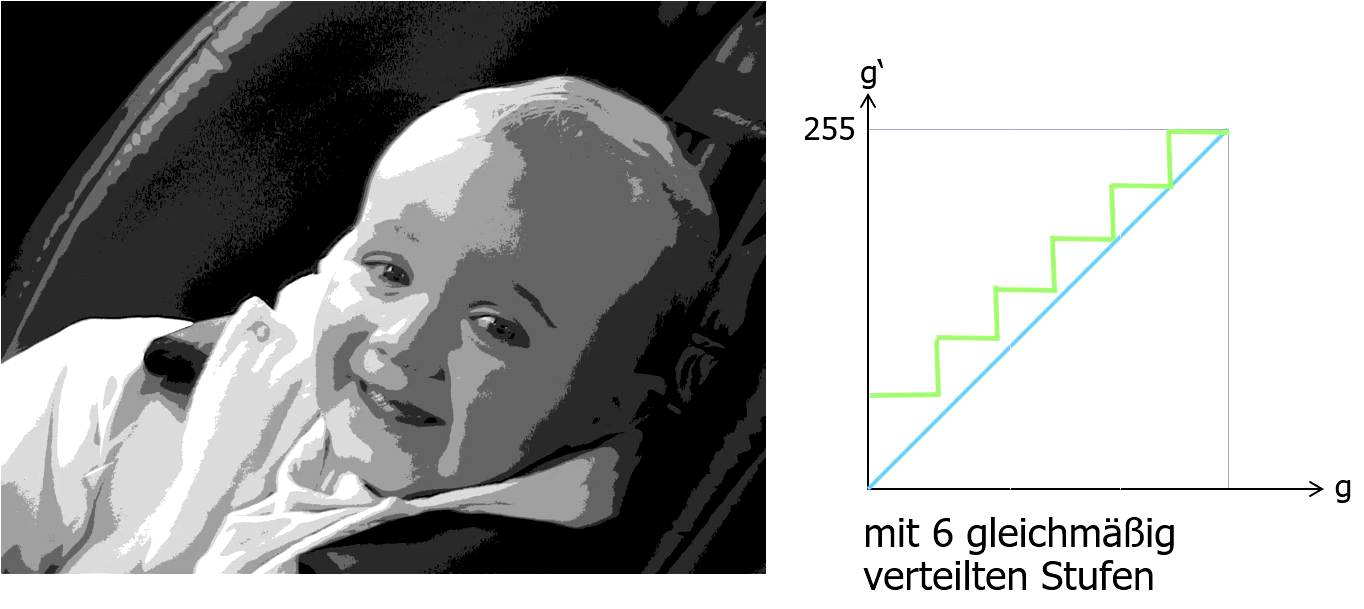
\includegraphics[height=150px]{PunktoperationAequidensitenbild.png}

Bei einem Äquidensitenbild wird der Wertebereich auf einige (im Beispiel 6) gleich weit voneinander entfernte Werte eingeschränkt. Das entspricht einer Biniarisierung mit einem Wertebereich mit mehr als 2 Elementen. Je mehr verschiedene Farbwerte genutzt werden, desto weniger auffallend ist diese lineare Grauwerttransformation. Diese Transformation findet Anwendung beim Drucken. Denn hier stehen eventuell nicht alle Farbwerte zur Verfügung. Deshalb müssen dann einige benachbarte Farbwerte auf die selbe Druckerfarbe abgebildet werden.

\subsubsection{Kontrastveränderung}

\includegraphics[height=150px]{KontrasterhöhungVorher.png} \hspace{200px}
\includegraphics[height=150px]{KontrasterhöhungNachher.png}

\includegraphics[height=100px]{KontrasterhöhungHistogrammVorher.png}
\hspace{150px}
\includegraphics[height=100px]{KontrasterhöhungHistogrammNachher.png}

Die Kontrastveränderung können wir zum Beispiel anwenden, um den Kontrast zu erhöhen, wenn ein Bild keinen vollen Kontrast hat, es also links oder rechts im Histogramm gibt, die nicht genutzt werden. Um das Bild auf einen vollen Kontrast zu transformieren muss die in schwarz eingezeichnete Grauwerttransformation durchgeführt werden. Es wird eine Gerade von $P_1=(g_{min}, g'_{MIN})$ bis $P_2=(g_{max}, g'_{MAX})$gezogen werden. Dabei sind $g_{min}$ und $g_{max}$ die minimalen und maximalen genutzten Grauwerte im Originalwert und $g'_{MIN}$ und  $g'_{MAX}$ die Grenzen des Wertebereichs im Ergebnisbild. der Bereich von $g'_{MIN}$ bis $g'_{MAX}$ bestimmt also welche Spanne von Werten das Ergebnisbild einnimmt und ist somit bei einer Erhöhung auf vollen Kontrast $g'_{MIN}=0$ und $g'_{MAX}=255$.\\
Man sieht, dass auf diese Weise Lücken im Histogramm entstehen, die Dynamik also abnimmt, die Entropie bleibt gleich, da es immernoch genau gleich viele unterschiedliche Pixelwerte mit der gleichen Verteilung gibt, nur haben sich die konkreten Werte geändert.\\

Beachte unbedingt die \hyperref[sec:Punktoperationen]{Einführung in die Punktoperationen}, um den Graphen richtig zu verstehen.

\subsection{Lokale Bildoperationen - Faltungsoperatoren}

\subsubsection{Faltungsmatrizen /-operatoren und deren Berechnung}
\label{sec:faltungsoperatoren}

\textbf{N4-Nachbarschaft}\\

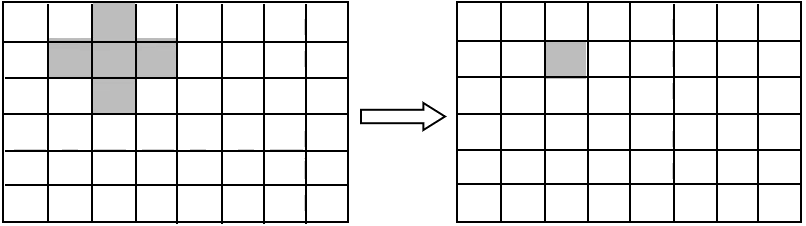
\includegraphics[height=70px]{N4Nachbarschaft.png}

\textbf{N8-Nachbarschaft}\\

\includegraphics[height=70px]{N8Nachbarschaft.png}

Lokale Bildoperationen sind Transformationen, bei denen für die Berechnung eines Pixels mehrere, nämlich sinnvoller Weise benachbarte, Pixel betrachtet werden. Bei den Nachbarschaftsbeziehung unterscheiden wir zwischen N4- und N8-Nachbarschaft, in welchen einem Pixel, das in der Mitte liegt, jeweils 4 oder 8 Nachbarn zugeordnet werden.\\
Haben wir uns für eine Nachbarschaftsform entschieden, dann müssen wir für jedes Pixel der ''Schablone'', auch Faltungsmatrix genannt, eine Gewichtung definieren. Bei der Berechnung eines Pixelwertes wird jeder Wert der Schablone mit dem Wert des jeweiligen Pixels multipliziert und dann alle so entstandenen Werte addiert. Zur Berechnung aller Pixel des Ergebnisbildes wird nun die Berechnung mit der Faltungsmatrix für jeden Pixel durchgeführt, also so, dass jedes Pixel des Originalbildes einmal in der Mitte der Faltunsmatrix liegt. Eine Ausnahme ist der äußere Rand des Originalbildes, für den es keine äußeren Nachbarn gibt. Deshalb wird der Rand weggelassen und das Ergebnisbild in beide Richtungen 2 Pixel kleiner.\\
In vielen Fällen ist der Wertebereich nicht mehr identisch mit dem Definitionsbereich $D \neq W$. In diesen Fällen müssen die Werte durch eine \hyperref[sec:Punktoperationen]{Lineare Transformation} wieder in den gültigen Bereich versetzt werden. Somit können wir lokale Operationen für Schwarz weiß Bilder anwenden. Wenn wir ein Farbbild haben führen wir die Berechnungen einfach für jeden Farbchannel durch. Im folgenden sehen wir die Berechnungsformel für eine N8-Faltungsmatrix:

$e(i, j) = \sum_{l=0}^{2} \sum_{k=0}^{2} [g(i-1+k, j-1+l) \cdot f(k, l)] $

Hierbei ist $g(a, b)$ der Wert des Pixels der Faltungsmatrix in der Zeil $a$ und der Spalte $b$. $f(a, b)$ ist der Wert des Pixels im Originalbild in der Zeile $a$ und der Spalte $b$. $e(i, j)$ ist der Wert des Pixels in der Zeile i und der Spalte b.\\
Die Summenzeichen sorgen dafür, dass wie mit einer verschachtelten for-Schleife über alle 9 Pixel der Faltungsmatrix iteriert wird.\\

Nun werden wir einige Beispiele für Faltungmatrizen sehen.

\subsubsection{Identität}

$
    I
    =
    \begin{pmatrix}
        0 & 0 & 0 \\
        0 & 1 & 0 \\
        0 & 0 & 0 \\
    \end{pmatrix}
$

Die Identität ist die Faltungsmatrix bei der nur der Wert des inneren Pixels beachtet wird. Dadurch bildet sie das Originalbild auf sich selbst ab und ist identisch mit der Punktoperation $g'(i,j) = g(i,j)$

\subsubsection{Glättungsfilter / Box-Filter / Mittelwertoperator}
\label{sec:mean-operator}

$
    A
    =
    \begin{pmatrix}
        1 & 1 & 1 \\
        1 & 1 & 1 \\
        1 & 1 & 1 \\
    \end{pmatrix}
$

\includegraphics[height=50px]{Glaettungsfilter.png}

Bei diesem einfachen Glättungsfilter wird jedes Pixel der Faltungsmatrix gleich stark Gewichtet. Dabei entsteht im Bild eine Unschärfe oder Glättung, weil die benachbarten Pixel verschwimmen. Allerdings entstehen um Kanten herum sogenannte \textbf{ringing artifacts}. Das sind Pixel, die um die Kanten herum liegen und den gleichen Farbwert wie die Kante haben. Somit wird es schwer die Schrift zu lesen.

\subsubsection{Gauß-Filter}

$
    A
    =
    \begin{pmatrix}
        1 & 2 & 1 \\
        2 & 4 & 2 \\
        1 & 2 & 1 \\
    \end{pmatrix}
$

\includegraphics[height=50px]{GaußFilter.png}

Der Gauß-Filter ist eine Glättungsfunktion, bei der die Gewichtung der inneren Pixel höher ist. Dadurch wird das Bild zwar geglättet, aber markante Punkte bleiben erkenntbar. Im Gegensatz zum normalen Glättungsfilter können wir hier die Schrift des damit erzeugten Bildes noch besser lesbar und die linien sind besser erkennbar.

\subsubsection{Differenzoperator \& Verständnis für die Ableitung}
\label{sec:difference-operator}

$
    A
    =
    \begin{pmatrix}
        0 & 0  & 0 \\
        0 & -1 & 1 \\
        0 & 0  & 0 \\
    \end{pmatrix}
    ,
    B
    =
    \begin{pmatrix}
        0  & 0 & 0 \\
        -1 & 1 & 0 \\
        0  & 0 & 0 \\
    \end{pmatrix}
    ,
    C
    =
    \begin{pmatrix}
        0 & -1 & 0 \\
        0 & 1  & 0 \\
        0 & 0  & 0 \\
    \end{pmatrix}
    ,
    D
    =
    \begin{pmatrix}
        0 & 0  & 0 \\
        0 & -2 & 1 \\
        0 & 1  & 0 \\
    \end{pmatrix}
$

\vspace{5px}

Der Differenzoperator hat seinen Namen davon, dass er differenziert also die Ableitung bildet. Dazu muss man sich nebeneinanderliegende Pixel zunächst als Funktion vorstellen, wobei jeder Pixelwert ein Funktionswert ist. Die Ableitung kann berechnet werden, indem für jeden Pixel die Steigung berechnet wird. Da wir es mit einem diskreten Definitionsbereich zu tun haben ist die Berechnung der Steigung in einem Punkt sehr einfach. Wir subtrahieren die Differenz der Funktionswerte (Pixelwerte) von benachbarten x-Werten (Pixeln) und Teilen durch deren Differenz der x-Werte. Da die Pixel benachbart sind ist ihre Differenz auf der x-Achse 1, wodurch die Division entfällt. Mit dieser Vorstellung sollte klar sein, dass $A$ und $B$ das identische Ergebnis, nämlich die Zeilenweise Ableitung bilden. $C$ bildet die spaltenweise Ableitung. $D$ bildet die Ableitung in Zeilen- und Spaltenrichtung, was einer hinternanderausführung von $A$ und $C$ entspricht. Da die Anwendung der Transformation auf eine Summe herausläuft können wir die Summe auch in der Matrix $D$ zusammenfassen.\\

Die Differenzoperatoren haben die Eigenschaft, dass Ergebnispixel stark positive Werte annehmen, wenn im Bild eine Kante von dunkel nach hell sichtbar war, stark negative Werte annehmen, wenn eine Kante von hell nach dunkel war und 0 sind, wenn benachbarte Pixel den gleichen Farbwert hatten. Somit wird klar, dass starke Kontraste hervorgehoben werden und schwache Kontraste weiter gedämpft werden.\\

Der Wertebereich von Differenzoperatoren ist grundlegend ungültig. Für $A$ ist er z.B. [-255, 255]. Um den Wertebereich wieder in den gültigen bereich zu transformieren wird eine \hyperref[sec:Punktoperationen]{lineare Transformation} durchgeführt, die zunächst den Wertebereich auf die selbe Mächtigkeit bringt, d.h. $|W|=256$ und dann auf [0, 255] verschiebt. Im Falle von $A$ wäre das dann die lineare Transformationsfunktion $f(x)=0.5x \cdot 128$

\subsubsection{Prewitt-Operator}

$
    A
    =
    \begin{pmatrix}
        -1 & 0 & 1 \\
        -1 & 0 & 1 \\
        -1 & 0 & 1 \\
    \end{pmatrix}
    ,
    B
    =
    \begin{pmatrix}
        -1 & -1 & -1 \\
        0  & 0  & 0  \\
        1  & 1  & 1  \\
    \end{pmatrix}
$

\vspace{5px}

Der Prewitt-Operator ist im Grunde nur eine Abwandlung des Differenzoperators. Hier wird sozusagen der Sichbereich erweitert.

\subsubsection{Sobel-Operator}
\label{sec:sobel-operator}

$
    A
    =
    \begin{pmatrix}
        -1 & 0 & 1 \\
        -2 & 0 & 2 \\
        -1 & 0 & 1 \\
    \end{pmatrix}
    ,
    B
    =
    \begin{pmatrix}
        -1 & -2 & -1 \\
        0  & 0  & 0  \\
        1  & 2  & 1  \\
    \end{pmatrix}
$

Der Sobel-Operator ist wiederum eine Variation des Prewitt-Operators.

\subsubsection{Laplace-Operator}

$
    A
    =
    \begin{pmatrix}
        0 & 1  & 1 \\
        1 & -4 & 1 \\
        0 & 1  & 0 \\
    \end{pmatrix}
$

\vspace{5px}

Der Laplace-Operator bildet die 2. Ableitung in Zeilen- und in Spaltenrichtung. Wir sehen also, dass der Laplace-Operator entsteht, wenn wir von den \hyperref[sec:difference-operator]{Differenzoperatoren} 2 spaltenweise Operatoren und 2 zeilenweise Operatoren addieren. Wir könnten das gleiche Ergebnis auch mit einer nicht-punktsymmetrischen Matrix erzielen, indem wir z.B. die \hyperref[sec:difference-operator]{Matrix $D$} 2 mal anwenden, also alle Werte elementweise mit 2 multiplizieren.

\subsubsection{Kantenhervorhebung bzw. Schärfungsfilter}
Die Kantenhervorhebung nimmt einen Kantendetektor (meist Laplace) und gibt dem inneren Pixel eine beliebige Wertigkeit $n$. Somit lässt sich das aktuelle Pixel stärker gewichten. Auf diese Weise kann ein Filterergebnis mit dem Originalbild vermischt werden. Je größer $n$ gewählt wird, desto mehr fällt das Originalbild ins Gewicht.\\
Beispiel für den kantenhervorhebenden Laplace-Filter:


$
    A
    =
    \begin{pmatrix}
        0  & -1    & -1 \\
        -1 & n + 4 & -1 \\
        0  & -1    & 0  \\
    \end{pmatrix}
$

\includegraphics[height=100px]{ausgangsbild.png}
\includegraphics[height=100px]{kantenhervohebung.png}

\includegraphics[width=400px]{relief-laplace-filter.png}

\subsubsection{Relief-Filter}

$
    A
    =
    \begin{pmatrix}
        -2 & -1 & 0 \\
        -1 & 1  & 1 \\
        0  & 1  & 2 \\
    \end{pmatrix}
$

\includegraphics[height=100px]{ausgangsbild.png}
\includegraphics[height=100px]{relif-filter.png}

\subsection{Lokale Bildoperatoren - Rangfolgeoperatoren}

\subsubsection{Rangfolgeoperatoren und deren Berechnung}

Rangfolgeoperatoren sind grundlegend ähnlich wie Faltungsoperatoren. Daher empfiehlt es sich das Kapitel \hyperref[sec:faltungsoperatoren]{Faltungsoperatoren} als Einstieg zu lesen. Bei Rangfolgeoperatoren wird nämlich ebenfalls zunächst eine Nachbarschaftsbeziehung gewählt und die entstandene Matrix pixelweise über das Bild bewegt, um den Wert für das mittlere Pixel zu berechnen. Die Berechnung des Ergebnispixels erfolgt aber nicht über eine kumulierte Multiplikation, sonder über eine Auswahl genau eines Wertes aus den eingehenden Pixelwerten:\\

Wir betrachten das Beispiel einer N8-Nachbarschaft, also einer 3x3-Matrix.
\begin{enumerate}
    \item Bei der Berechnung eines Pixel werden zunächst die Werte der Eingangspixel der größe nach geordnet.
    \item Dann wird einer der Werte nach einer gewissen Vorschrift ausgewählt. Konkrete Vorschriften folgen im nächsten \hyperref[sec:types-of-ranking-operators]{Teilkapitel}.
\end{enumerate}

\subsubsection{Arten von Rangfolgeoperatoren}
\label{sec:types-of-ranking-operators}

Wir wollen hier 3 verschiedene Rangfolgeoperatoren kennenlernen und beispielhaft ihre Auswirkungen betrachten:

\textbf{Medianoperator}\\

\includegraphics[height=150px]{medianoperator1.png}
\includegraphics[height=150px]{medianoperator2.png}

Beim Medianoperator wird der Median unserer Eingangswerte, also der mittlere Wert der Rangfolge, übernommen. Das Ergebnis ist, dass Ecken abgerundet werden, aber im Gegensatz zum \hyperref[sec:mean-operator]{Mittelwertoperator} keine verschwommenen Kanten entstehen, da keine Werte gemischt werden.\\


\textbf{Erosion}\\

\includegraphics[height=150px]{erosion.png}

Bei der Erosion wird der dunkelste, also geringste Wert der Rangfolge übernommen. Das bedeutet, dass helle Teile an ihren Kanten, also dort wo sie auf dunklere Teile treffen, kleiner werden und dunkle Teile größer. Falls ein helles Objekt kleiner als die Rangfolgenmatrix ist verschwindet es komplett, da für jeden Punkt mindestens ein umliegender Punkt heller als das Objekt ist.\\

\textbf{Dilatation}\\

\includegraphics[height=150px]{diliatation.png}

Hier wird der hellste, also höchste Wert übernommen, dementsprechend das logische Gegenstück zur Erosion.

\subsubsection{Anwendung und Kombination von Rangfolgeoperatoren}

Die Anwendung von Rangfolgeoperatoren kann gut benutzt werden, um die Komplexität eines Bildes so stark zu vermindern, dass nur noch die relevanten Teile vorhanden sind. Solche Bilder können dann als Input für KIs dienen, welche die Bilder dann auswerten können. Wir benennen die folgenden Kombinationen:
\begin{itemize}
    \item \textbf{Opening:} erst Erosion dann Dilatation
    \item \textbf{Closing:} erst Dilatation dann Erosion
\end{itemize}

Wir wollen an einem Beispiel nun zeigen, wie wir ein Bild verarbeiten können. Dazu wenden wir folgende Schritte an:
\begin{itemize}
    \item Biniarisierung mit Schwellwert 225
    \item Closing\\
          \begin{itemize}
              \item Dilatation
              \item Erosion
          \end{itemize}
    \item Opening\\
          \begin{itemize}
              \item Erosion
              \item Dilatation
          \end{itemize}
\end{itemize}

\vspace{5px}

\includegraphics[height=100px]{pfeil1.png}
\includegraphics[height=100px]{pfeil2.png}
\includegraphics[height=100px]{pfeil3.png}
\includegraphics[height=100px]{pfeil4.png}
\includegraphics[height=100px]{pfeil5.png}

Damit Objekte gleich groß bleiben müssen genau so viele Erosionen wie Dilatationen durchgeführt werden. Dies gilt unter der vorraussetzungen, dass die Objekte vor jeder Iteration noch mindestens so groß wie die Rangfolgenmatrix sind, damit sie nicht vollständig verschwinden.

\subsection{Algorithmen}

\subsubsection{Canny-Edge-Detector}
\label{sec:canny-edge-detector}

Der Canny-Edge-Detector ist ein Algorithmus zur Kantenerkennung, der aus mehreren Faltungsoperationen besteht und dazu führen soll, dass das Ergebnisbild im Idealfall nur noch die Kanten des Eingangsbild enthält. Den Algorithmus kann man in 5 Schritte unterteilen, die wir hier einmal vorgestellt und erklärt werden sollen:

\subsubsection*{(i) Konvertierung zum Graubild}

\includegraphics[height=200px]{canny-1.png}
\includegraphics[height=200px]{canny-2.png}

Dieser Schritt ist notwendig, da der Algorithmus nur für die arbeit mit einem Farbkanal definiert ist.

\subsubsection*{(ii) Berechnung des Gradientenfeldes}

\includegraphics[height=200px]{canny-3.png}
\includegraphics[height=200px]{canny-4.png}

Mit Gradientenfeld ist die Ableitung, also die Steigung (also somit das Gefälle -\textless Gradient) gemeint (siehe \hyperref[sec:difference-operator]{Differenzierungsoperator}). Wir berechnen diese Gradienten sowohl horizontal als auch vertikal und benutzen dafür konkret den \hyperref[sec:sobel-operator]{Sobel-Operator}

\subsubsection*{(iii) Bestimmung des Betrags der Gradientenvektoren}

\includegraphics[height=200px]{canny-5.png}

Das Ziel dieses Schrittes ist es die vertikale und die horizontale Information zusammenzufügen. Dazu wird aus den beiden Werten für jedes Pixel ein 2-dimensionaler Vektor gebildet. Dann wird der Betrag (also die Länge) dieses Vektors berechnet. Das Ergebnis ist der neue Wert des Pixels.



\subsubsection*{(iv) Ausdünnen der Kanten - Non Maximum Suppression}

\includegraphics[height=200px]{canny-6.png}

Hiermit soll sichergestellt werden, dass jede Kante nur 1 pixel breit ist. Dazu wird eine 3x3-Matrix über das Bild verschoben, und jeweils alle Nicht-Maxima, d.h. alle 8 Werte außer dem größten Wert, auf 0 gesetzt.

\subsubsection*{(v) Hysterese}

\includegraphics[height=150px]{canny-7.png}

Die Hysterese ist eine Art von \hyperref[sec:biniarisierung]{Biniarisierung}. Das heißt, dass wir mittels Schwellwerten einen Wert entweder behalten wollen (im Ergebnisbild weiß) oder entfernen wollen (im Ergebnisbild schwarz = Hintergrund). Im Gegensatz zur normalen Biniarisierung mit einem einzigen Schwellwert werden bei der Hysterese 2 Schwellwerte $ T_{1} < T_{2} $ verwendet.\\
Im ersten Schritt wird ein Pixel, wenn sein Wert größer als $T_{2}$ ist, als Bestandteil einer starken Kante eingestuft. Wenn ein Wert eines Pixels größer als $ T_{1} $ aber kleiner als $T_{2}$ ist, dann wird der Pixel als Bestandteil einer schwachen Kante eingestuft.\\
Im zweiten Schritt werden zunächst alle starken Kanten übernommen. Schwache Kanten werden nur dann übernommen, wenn sie starke Kanten berühren.\\

Das Ziel der Hysterese ist es nicht relevante schwache Kanten zu eliminieren. Im folgenden Ergebnisbild kann man sehen, dass z.B. die schwachen Kanten in der rechten unteren Ecke nicht übernommen wurden:

\includegraphics[height=200px]{canny-8.png}

\subsubsection{Hough-Transformation}

Die Hough-Transformation ist ein Verfahren zur Erkennung von Geraden, Kreisen oder anderen parametrisierbaren geometrischen Figuren in Bildern. Dabei ist schon bekannt welche Figur man erkennen möchte, man will aber die Position und Größe genau lokalisieren können. Wir wollen uns dies anhand von der Erkennung von Geraden ansehen.\\

\includegraphics[height=200px]{hough-transformation-1.png}

Zunächst benötigen wir ein Eingangsbild, das die von uns zu erfassende Figur - die Gerade - möglichst eindeutig enthält. Um solch ein Bild aus einem realen Bild zu extrahieren können andere Algorithmen, wie z.B. der \hyperref[sec:canny-edge-detector]{Canny-Edge-Detector} verwendet werden.\\
Dann müssen wir festlegen mit welchen Parametern wir die Gerade darstellen wollen. Naheliegend wäre die Steigung und der y-Achsenabschnitt (klassische Darstellung linearer Funktionen). Doch hier entsteht das Problem, dass senkrechte Geraden nicht dargestellt werden können, da sie jedem x-Wert mehrere y-Werte zuordnen würde, also sozusagen eine ''unendliche Steigung'' hätte. Stattdessen können wir die Gerade auch mittels einem Winkel $\theta$ und einer Länge $p$ darstellen. Wir zeichnen eine Orthogonale zur Gerade, die durch den Ursprung verläuft. $\theta$ ist dann der Winkel der Orthogonalen zur x-Achse und $p$ die Länge dieser Orthogonalen. Der entstandene 2-dimensionale Vektorraum (im Grunde ein einfaches 2-dimensionales Koordinatensystem) wird auch Hough-Raum genannt. Jeder konkrete Punkt im Hough-Raum stellt also eine Gerade im Eingabebild dar.\\
Nun iterieren wir über alle relevanten Pixel des Eingangsbildes (die ja alle zu Kanten gehören, da das Bild entsprechend vorverarbeitet wurde) und finden errechnen für jeden Pixel alle möglichen Geraden, die diesen Punkt laufen. Mathematisch gesehen sind das natürlich unendlich viele Geraden, aber da unser Eingabebild nur begrenzt viele Pixel, also eine begrenzte Genauigkeit besitzt ist auch die Anzahl der verschiedenen Geraden im Bild endlich. Für jede dieser Geraden wird ein Wert, der dem entsprechende Punkt im Hough-Raum zugeordnet wird, inkrementiert. Es wird also sozusagen für diesen Punkt gevotet. Wir können die Werte, welche den Punkten im Hough-Raum zugeordnet werden dan mit Helligkeitswerten darstellen. Wenn wir das für alle Punkte durchgeführt haben, haben die Punkte im Hough-Raum, zu denen es am meisten Pixel im Eingangsbild gibt, die zu dieser Geraden gehören könnten, den höchsten Wert. Wenn man nun die Hochpunkte der Werte im Hough-Raum findet, so erhält man also die genauen Gleichungen für die Geraden im Bild und hat somit die Geraden identifiziert.

\includegraphics[height=200px]{hough-transformation-2.png}

\subsubsection{Harris-Corner-Edge-Detection}

Harris-Corner-Edge-Detection ist ein Verfahren zum Erkennen von Interest-Points. Interest-Points, oder auch Feature-Points genannt, sind Punkte, die man in verschiedenen Bildern der gleichen Szene oder des gleichen Objekts gut wiedererkennen kann. Die Erkennung von Interest-Points ermöglicht es z.B. automatisierte Objektverfolgung u.v.m. zu implementieren. Interest-Points sind also besonders signifikante Punkte, die möglichst aus verschiedenen Perspektiven trotzdem ähnlich aussehen.\\

\includegraphics[height=125px]{harris-corner-edge.png}

Der Harris-Corner-Edge-Detector versucht signifikante Punkte zu finden, indem er misst wie verschieden ein Bereich von seinem Umfeld ist. Dabei wird gemessen wie groß der Unterschied der Pixelwerte ist, wenn man eine lokale-Nachbarschaftsmatrix um jeweils ein Pixel in jede Richtung verschiebt. Man erkennt im Beispiel:
\begin{itemize}
    \item \textbf{Im erstem Bild} verändern sich die Pixelwerte überhaupt nicht
    \item \textbf{Im zweiten Bild} verändern sich die Pixelwerte bei der vertikalen Verschiebung nicht
    \item \textbf{Im dritten Bild} verändern sich die Pixelwerte in jedem Fall $\rightarrow$ Iterest-Point gefunden
\end{itemize}

\subsubsection{SIFT - Scale-invariant Feature Transform}
\label{sec:sift}
SIFT ist ein Feature-Point-Detektionsalgorithmus, der eine lokale Umgebung auf eine Menge von Vektoren, sog. feature-vectors, abbildet. Das besondere der entstandenen feature-vectors ist, das sie so berechnet sind, dass sie weitestgehend unabhängig von Translation, Skalierung und Rotation des Objektes sind, das sie beschreiben. Dadurch ergeben sich für das gleiche Objekt aus einer anderen Perspektive die gleichen feature-vectors. Sucht man nur ein bestimmtes bekanntes Objekt in einem Bild, dann kann man es anhand seiner Menge an feature-vectors ermitteln. Auf die Details der Berechnung soll hier nicht näher eingegangen werden.

\subsubsection{Template Matching}

Wir haben bereits die Hough-Transformation kennengelernt, um Geometrische Formen in einem Bild zu erkennen, wie etwa Linien oder Kreise. Wenn wir aber komplexere Objekte erkennen möchten, die sich nicht einfach durch mathematische Zusammenhänge beschreiben lassen, müssen wir Template Matching betreiben. Der Input, den ein Template-Matching-Algorithmus verarbeitet sind ein Eingabebild, in dem gesuchte werden soll und ein Template, das angibt nach was gesucht werden soll. Der gewünschte Output ist dann die Position des gesuchten Objektes im Bild. \\

\includegraphics[height=150px]{TemplateMatching3.png}

\includegraphics[height=150px]{templateMatching1.png}
\includegraphics[height=150px]{TemplateMatching2.png}

Um das zu bewerkstelligen, kann für jede Möglichkeit das Template auf dem Eingabebild zu platzieren berechnet werden, wie hoch die Abweichung ist. Wenn der Fehler unter einem gewissen Schwellwert liegt, kann man festlegen, dass ein Match erkannt werden soll. Für die Berechnung des Fehlers kann z.B. der Betrag der Summe der pixelweisen Differenzen $F_{1}$ herangezogen werden, oder auch die Summe der Quadrate der pixelweisen Differenzen $F_{2}$:

\[
    F_{1} = \sum_{k=0}^{n}|P_{0}(x, y) - P_{1}(x, y)|
\]

\[
    F_{2} = \sum_{k=0}^{n}(P_{0}(x, y) - P_{1}(x, y))^{2}
\]

Die Schwierigkeiten beim Template Matching sind Abweichungen der Größe, Rotation, veränderte Belichtung und anderer Hintergrund des gesuchten Bereichs im Eingabebild. Es entstehen also insgesamt sehr viele Möglichkeiten, wie das Template im Bild versteckt werden kann. Im Gegensatz zum Brute-Force-Ansatz, bei dem wir alle Möglichkeiten durchprobieren würden, also etwa mit verschiedenen Drehwinkeln und Größen des Templates, gibt es auch noch den Ansatz mit Deep-Learning-Algorithmen. Bei diesem Ansatz berechnet der Algorithmus Feature-Vektoren, die im besten Fall weitestgehend invariant im Bezug auf verschiedene Transformationen, Clutter im Bild und veränderte Lichtverhältnisse sind.

\subsubsection{Image Stitching}

\includegraphics[height=150px]{imageStitching.png}

\includegraphics[height=150px]{featureMatches.png}

\includegraphics[height=150px]{panorama.png}

Beim Image Stitching geht es darum aus mehreren Teilbildern ein gemeinsames Bild zu erzeugen. Ein gutes Beispiel ist die Panorama-Funktion eines Handys, bei der man mehrere Bilder aufnimmt, die dann zusammengefügt werden. Die Grundlegende Herangehensweise ist die folgende:

\begin{enumerate}
    \item \textbf{Identifizieren von Feature Points:}\\
          Zunächst müssen Feature Points, also markante Punkte im Bild, erkannt werden. Hierfür kann z.B. der \hyperref[sec:sift]{SIFT-Algorithmus} verwendet werden
    \item \textbf{Finden von Feature-Pairs:}\\
          Dann müssen Feature-Pairs, also Paare aus Feature-Points der beiden Bildern, die zu den selben Objekten gehören, gefunden werden
    \item \textbf{Berechnung der Homografie:}\\
          Basierend auf den Vektoren, die die Feature-Pairs verbinden kann eine Homografie berechnet werden. Die Homografie ist das Verhältnis der beiden Kamerapositionen der beiden Bilder.
    \item \textbf{Zusamenfügen der Bilder:}\\
          Die Bilder werden an geeigneter Stelle übereinandergelegt
    \item \textbf{Morphing:}\\
          Wenn wir im überlappenden Bereich einfach die Mittelwerte der Pixelwerte bilden führt dies zu einer Unschärfe. Das liegt daran, dass die Bilder auf verschiedenen Winkeln geschossen sind und die Bereiche also nicht komplett identisch aussehen. Wir haben also 2 leicht verschiedene Bilder und wir wollen das Bild errechnen, dass sich im Übergang von einem Bild zum anderen Befindet. Den Prozess des findens dieses Übergansbildes nennt man Morphing.
\end{enumerate}
\end{document}
